\documentclass[twoside]{book}

% Packages required by doxygen
\usepackage{fixltx2e}
\usepackage{calc}
\usepackage{doxygen}
\usepackage[export]{adjustbox} % also loads graphicx
\usepackage{graphicx}
\usepackage[utf8]{inputenc}
\usepackage{makeidx}
\usepackage{multicol}
\usepackage{multirow}
\PassOptionsToPackage{warn}{textcomp}
\usepackage{textcomp}
\usepackage[nointegrals]{wasysym}
\usepackage[table]{xcolor}

% Font selection
\usepackage[T1]{fontenc}
\usepackage[scaled=.90]{helvet}
\usepackage{courier}
\usepackage{amssymb}
\usepackage{sectsty}
\renewcommand{\familydefault}{\sfdefault}
\allsectionsfont{%
  \fontseries{bc}\selectfont%
  \color{darkgray}%
}
\renewcommand{\DoxyLabelFont}{%
  \fontseries{bc}\selectfont%
  \color{darkgray}%
}
\newcommand{\+}{\discretionary{\mbox{\scriptsize$\hookleftarrow$}}{}{}}

% Page & text layout
\usepackage{geometry}
\geometry{%
  a4paper,%
  top=2.5cm,%
  bottom=2.5cm,%
  left=2.5cm,%
  right=2.5cm%
}
\tolerance=750
\hfuzz=15pt
\hbadness=750
\setlength{\emergencystretch}{15pt}
\setlength{\parindent}{0cm}
\setlength{\parskip}{3ex plus 2ex minus 2ex}
\makeatletter
\renewcommand{\paragraph}{%
  \@startsection{paragraph}{4}{0ex}{-1.0ex}{1.0ex}{%
    \normalfont\normalsize\bfseries\SS@parafont%
  }%
}
\renewcommand{\subparagraph}{%
  \@startsection{subparagraph}{5}{0ex}{-1.0ex}{1.0ex}{%
    \normalfont\normalsize\bfseries\SS@subparafont%
  }%
}
\makeatother

% Headers & footers
\usepackage{fancyhdr}
\pagestyle{fancyplain}
\fancyhead[LE]{\fancyplain{}{\bfseries\thepage}}
\fancyhead[CE]{\fancyplain{}{}}
\fancyhead[RE]{\fancyplain{}{\bfseries\leftmark}}
\fancyhead[LO]{\fancyplain{}{\bfseries\rightmark}}
\fancyhead[CO]{\fancyplain{}{}}
\fancyhead[RO]{\fancyplain{}{\bfseries\thepage}}
\fancyfoot[LE]{\fancyplain{}{}}
\fancyfoot[CE]{\fancyplain{}{}}
\fancyfoot[RE]{\fancyplain{}{\bfseries\scriptsize Generated by Doxygen }}
\fancyfoot[LO]{\fancyplain{}{\bfseries\scriptsize Generated by Doxygen }}
\fancyfoot[CO]{\fancyplain{}{}}
\fancyfoot[RO]{\fancyplain{}{}}
\renewcommand{\footrulewidth}{0.4pt}
\renewcommand{\chaptermark}[1]{%
  \markboth{#1}{}%
}
\renewcommand{\sectionmark}[1]{%
  \markright{\thesection\ #1}%
}

% Indices & bibliography
\usepackage{natbib}
\usepackage[titles]{tocloft}
\setcounter{tocdepth}{3}
\setcounter{secnumdepth}{5}
\makeindex

% Hyperlinks (required, but should be loaded last)
\usepackage{ifpdf}
\ifpdf
  \usepackage[pdftex,pagebackref=true]{hyperref}
\else
  \usepackage[ps2pdf,pagebackref=true]{hyperref}
\fi
\hypersetup{%
  colorlinks=true,%
  linkcolor=blue,%
  citecolor=blue,%
  unicode%
}

% Custom commands
\newcommand{\clearemptydoublepage}{%
  \newpage{\pagestyle{empty}\cleardoublepage}%
}

\usepackage{caption}
\captionsetup{labelsep=space,justification=centering,font={bf},singlelinecheck=off,skip=4pt,position=top}

%===== C O N T E N T S =====

\begin{document}

% Titlepage & ToC
\hypersetup{pageanchor=false,
             bookmarksnumbered=true,
             pdfencoding=unicode
            }
\pagenumbering{roman}
\begin{titlepage}
\vspace*{7cm}
\begin{center}%
{\Large Prometheus frontier explorer }\\
\vspace*{1cm}
{\large Generated by Doxygen 1.8.11}\\
\end{center}
\end{titlepage}
\clearemptydoublepage
\tableofcontents
\clearemptydoublepage
\pagenumbering{arabic}
\hypersetup{pageanchor=true}

%--- Begin generated contents ---
\chapter{Hierarchical Index}
\section{Class Hierarchy}
This inheritance list is sorted roughly, but not completely, alphabetically\+:\begin{DoxyCompactList}
\item \contentsline{section}{Frontier\+Explorer}{\pageref{classFrontierExplorer}}{}
\item \contentsline{section}{Map}{\pageref{classMap}}{}
\item \contentsline{section}{Map\+Node}{\pageref{classMapNode}}{}
\item Test\begin{DoxyCompactList}
\item \contentsline{section}{Frontier\+Explorer\+Test}{\pageref{classFrontierExplorerTest}}{}
\item \contentsline{section}{Map\+Node\+Test}{\pageref{classMapNodeTest}}{}
\item \contentsline{section}{Map\+Test}{\pageref{classMapTest}}{}
\end{DoxyCompactList}
\item \contentsline{section}{Test\+Sub\+Pub}{\pageref{classTestSubPub}}{}
\end{DoxyCompactList}

\chapter{Class Index}
\section{Class List}
Here are the classes, structs, unions and interfaces with brief descriptions\+:\begin{DoxyCompactList}
\item\contentsline{section}{\hyperlink{classFrontierExplorer}{Frontier\+Explorer} \\*Frontier\+Exploration Class }{\pageref{classFrontierExplorer}}{}
\item\contentsline{section}{\hyperlink{classFrontierExplorerTest}{Frontier\+Explorer\+Test} \\*\hyperlink{classFrontierExplorerTest}{Frontier\+Explorer\+Test} Class }{\pageref{classFrontierExplorerTest}}{}
\item\contentsline{section}{\hyperlink{classMap}{Map} \\*\hyperlink{classMap}{Map} Class }{\pageref{classMap}}{}
\item\contentsline{section}{\hyperlink{classMapNode}{Map\+Node} \\*\hyperlink{classMapNode}{Map\+Node} Class }{\pageref{classMapNode}}{}
\item\contentsline{section}{\hyperlink{classMapNodeTest}{Map\+Node\+Test} \\*\hyperlink{classMapNodeTest}{Map\+Node\+Test} Class }{\pageref{classMapNodeTest}}{}
\item\contentsline{section}{\hyperlink{classMapTest}{Map\+Test} \\*\hyperlink{classMapTest}{Map\+Test} Class }{\pageref{classMapTest}}{}
\item\contentsline{section}{\hyperlink{classTestSubPub}{Test\+Sub\+Pub} \\*\hyperlink{classTestSubPub}{Test\+Sub\+Pub} Class }{\pageref{classTestSubPub}}{}
\end{DoxyCompactList}

\chapter{File Index}
\section{File List}
Here is a list of all documented files with brief descriptions\+:\begin{DoxyCompactList}
\item\contentsline{section}{/home/hbk/\+Desktop/\+Software\+Development/\+Final\+Project/rosworld/src/prometheus\+\_\+frontier\+\_\+explorer/include/\hyperlink{FrontierExplorer_8hpp}{Frontier\+Explorer.\+hpp} \\*\hyperlink{classFrontierExplorer}{Frontier\+Explorer} header file }{\pageref{FrontierExplorer_8hpp}}{}
\item\contentsline{section}{/home/hbk/\+Desktop/\+Software\+Development/\+Final\+Project/rosworld/src/prometheus\+\_\+frontier\+\_\+explorer/include/\hyperlink{Map_8hpp}{Map.\+hpp} \\*\hyperlink{classMap}{Map} class header file }{\pageref{Map_8hpp}}{}
\item\contentsline{section}{/home/hbk/\+Desktop/\+Software\+Development/\+Final\+Project/rosworld/src/prometheus\+\_\+frontier\+\_\+explorer/include/\hyperlink{MapNode_8hpp}{Map\+Node.\+hpp} \\*\hyperlink{classMapNode}{Map\+Node} class header file }{\pageref{MapNode_8hpp}}{}
\item\contentsline{section}{/home/hbk/\+Desktop/\+Software\+Development/\+Final\+Project/rosworld/src/prometheus\+\_\+frontier\+\_\+explorer/src/\hyperlink{FrontierExplorer_8cpp}{Frontier\+Explorer.\+cpp} \\*\hyperlink{classFrontierExplorer}{Frontier\+Explorer} class }{\pageref{FrontierExplorer_8cpp}}{}
\item\contentsline{section}{/home/hbk/\+Desktop/\+Software\+Development/\+Final\+Project/rosworld/src/prometheus\+\_\+frontier\+\_\+explorer/src/\hyperlink{Map_8cpp}{Map.\+cpp} \\*\hyperlink{classMap}{Map} class implementation file }{\pageref{Map_8cpp}}{}
\item\contentsline{section}{/home/hbk/\+Desktop/\+Software\+Development/\+Final\+Project/rosworld/src/prometheus\+\_\+frontier\+\_\+explorer/src/\hyperlink{MapNode_8cpp}{Map\+Node.\+cpp} \\*\hyperlink{classMapNode}{Map\+Node} class implementation file }{\pageref{MapNode_8cpp}}{}
\item\contentsline{section}{/home/hbk/\+Desktop/\+Software\+Development/\+Final\+Project/rosworld/src/prometheus\+\_\+frontier\+\_\+explorer/test/\hyperlink{FrontierExplorerTest_8cpp}{Frontier\+Explorer\+Test.\+cpp} \\*Test for \hyperlink{classFrontierExplorer}{Frontier\+Explorer} class file }{\pageref{FrontierExplorerTest_8cpp}}{}
\item\contentsline{section}{/home/hbk/\+Desktop/\+Software\+Development/\+Final\+Project/rosworld/src/prometheus\+\_\+frontier\+\_\+explorer/test/\hyperlink{MapNodeTest_8cpp}{Map\+Node\+Test.\+cpp} \\*Test for \hyperlink{classMapNode}{Map\+Node} class file }{\pageref{MapNodeTest_8cpp}}{}
\item\contentsline{section}{/home/hbk/\+Desktop/\+Software\+Development/\+Final\+Project/rosworld/src/prometheus\+\_\+frontier\+\_\+explorer/test/\hyperlink{MapTest_8cpp}{Map\+Test.\+cpp} \\*Test for \hyperlink{classMap}{Map} class file }{\pageref{MapTest_8cpp}}{}
\end{DoxyCompactList}

\chapter{Class Documentation}
\hypertarget{classFrontierExplorer}{}\section{Frontier\+Explorer Class Reference}
\label{classFrontierExplorer}\index{Frontier\+Explorer@{Frontier\+Explorer}}


Frontier\+Exploration Class.  




{\ttfamily \#include $<$Frontier\+Explorer.\+hpp$>$}

\subsection*{Public Member Functions}
\begin{DoxyCompactItemize}
\item 
\hyperlink{classFrontierExplorer_aeb9f6b222b5e31b8c41f41e04fece7b0}{Frontier\+Explorer} ()
\begin{DoxyCompactList}\small\item\em Default constructor for \hyperlink{classFrontierExplorer}{Frontier\+Explorer} class. \end{DoxyCompactList}\item 
\hyperlink{classFrontierExplorer_a4f855409482b23bb537505f5543c3e0d}{$\sim$\+Frontier\+Explorer} ()
\begin{DoxyCompactList}\small\item\em Destructor for \hyperlink{classFrontierExplorer}{Frontier\+Explorer} class. \end{DoxyCompactList}\item 
void \hyperlink{classFrontierExplorer_aacc7b104656ec07f8901abeae2d1b2c3}{process\+Occupancy\+Grid} (const nav\+\_\+msgs\+::\+Occupancy\+Grid\+::\+Const\+Ptr \&grid\+Msg)
\begin{DoxyCompactList}\small\item\em Callback function for processing Occupancy Grid. \end{DoxyCompactList}\item 
void \hyperlink{classFrontierExplorer_acdb01ab0862ad3d22b5c13e13edae821}{explore} ()
\begin{DoxyCompactList}\small\item\em Wrapper function to start frontier exploration. \end{DoxyCompactList}\item 
void \hyperlink{classFrontierExplorer_acdea468a554a1665ada8a9d47fdb12ad}{rotate360} ()
\begin{DoxyCompactList}\small\item\em Function to rotate turtle bot 360 degrees. \end{DoxyCompactList}\item 
int \hyperlink{classFrontierExplorer_acdb43fe4d75b89328499eaab690ef576}{get\+Nearest\+Cluster} (std\+::vector$<$ std\+::pair$<$ double, double $>$$>$ centers)
\begin{DoxyCompactList}\small\item\em Function to get nearest cluster. \end{DoxyCompactList}\item 
bool \hyperlink{classFrontierExplorer_a645d0985b5e21046af0864c6933b27cb}{check\+Reach\+Avoid} (std\+::pair$<$ double, double $>$ goal\+Point)
\begin{DoxyCompactList}\small\item\em Function to check if point is to be visited. \end{DoxyCompactList}\item 
void \hyperlink{classFrontierExplorer_a0c2bdfdf926178c67a521b30b98c798a}{move\+Turtle} (std\+::vector$<$ std\+::pair$<$ double, double $>$$>$ centers, int id)
\begin{DoxyCompactList}\small\item\em Function to navigate the turtlebot to cluster. \end{DoxyCompactList}\item 
void \hyperlink{classFrontierExplorer_a8a7b32fda86f272b5bb10b72485d6a20}{publish\+Frontier\+Points} (int count)
\begin{DoxyCompactList}\small\item\em Function to visualize all frontier points in Rviz. \end{DoxyCompactList}\item 
void \hyperlink{classFrontierExplorer_a4b4a64865166c3641d20496a0cab9b83}{visualize\+Cluster\+Centers} (std\+::vector$<$ std\+::pair$<$ double, double $>$$>$ centers, int id)
\begin{DoxyCompactList}\small\item\em Function to visualize all cluster centers in Rviz. \end{DoxyCompactList}\item 
void \hyperlink{classFrontierExplorer_aedf341ee2e9b63ee6e9adc7a7d8e3c44}{visualize\+Cluster\+Frontiers} ()
\begin{DoxyCompactList}\small\item\em Function to visualize frontiers segregated based on clusters in Rviz. \end{DoxyCompactList}\item 
void \hyperlink{classFrontierExplorer_a2a7e35e8b561d2d79c7ce3747b1ee07a}{visualize\+Reach\+Avoid} ()
\begin{DoxyCompactList}\small\item\em Function to visualize reach avoid regions in Rviz. \end{DoxyCompactList}\end{DoxyCompactItemize}


\subsection{Detailed Description}
Frontier\+Exploration Class. 

Class for frontier exploration. 

\subsection{Constructor \& Destructor Documentation}
\index{Frontier\+Explorer@{Frontier\+Explorer}!Frontier\+Explorer@{Frontier\+Explorer}}
\index{Frontier\+Explorer@{Frontier\+Explorer}!Frontier\+Explorer@{Frontier\+Explorer}}
\subsubsection[{\texorpdfstring{Frontier\+Explorer()}{FrontierExplorer()}}]{\setlength{\rightskip}{0pt plus 5cm}Frontier\+Explorer\+::\+Frontier\+Explorer (
\begin{DoxyParamCaption}
{}
\end{DoxyParamCaption}
)}\hypertarget{classFrontierExplorer_aeb9f6b222b5e31b8c41f41e04fece7b0}{}\label{classFrontierExplorer_aeb9f6b222b5e31b8c41f41e04fece7b0}


Default constructor for \hyperlink{classFrontierExplorer}{Frontier\+Explorer} class. 


\begin{DoxyParams}{Parameters}
{\em none} & \\
\hline
\end{DoxyParams}
\begin{DoxyReturn}{Returns}
none 
\end{DoxyReturn}
\index{Frontier\+Explorer@{Frontier\+Explorer}!````~Frontier\+Explorer@{$\sim$\+Frontier\+Explorer}}
\index{````~Frontier\+Explorer@{$\sim$\+Frontier\+Explorer}!Frontier\+Explorer@{Frontier\+Explorer}}
\subsubsection[{\texorpdfstring{$\sim$\+Frontier\+Explorer()}{~FrontierExplorer()}}]{\setlength{\rightskip}{0pt plus 5cm}Frontier\+Explorer\+::$\sim$\+Frontier\+Explorer (
\begin{DoxyParamCaption}
{}
\end{DoxyParamCaption}
)}\hypertarget{classFrontierExplorer_a4f855409482b23bb537505f5543c3e0d}{}\label{classFrontierExplorer_a4f855409482b23bb537505f5543c3e0d}


Destructor for \hyperlink{classFrontierExplorer}{Frontier\+Explorer} class. 


\begin{DoxyParams}{Parameters}
{\em none} & \\
\hline
\end{DoxyParams}
\begin{DoxyReturn}{Returns}
none 
\end{DoxyReturn}


\subsection{Member Function Documentation}
\index{Frontier\+Explorer@{Frontier\+Explorer}!check\+Reach\+Avoid@{check\+Reach\+Avoid}}
\index{check\+Reach\+Avoid@{check\+Reach\+Avoid}!Frontier\+Explorer@{Frontier\+Explorer}}
\subsubsection[{\texorpdfstring{check\+Reach\+Avoid(std\+::pair$<$ double, double $>$ goal\+Point)}{checkReachAvoid(std::pair< double, double > goalPoint)}}]{\setlength{\rightskip}{0pt plus 5cm}bool Frontier\+Explorer\+::check\+Reach\+Avoid (
\begin{DoxyParamCaption}
\item[{std\+::pair$<$ double, double $>$}]{goal\+Point}
\end{DoxyParamCaption}
)}\hypertarget{classFrontierExplorer_a645d0985b5e21046af0864c6933b27cb}{}\label{classFrontierExplorer_a645d0985b5e21046af0864c6933b27cb}


Function to check if point is to be visited. 


\begin{DoxyParams}{Parameters}
{\em std\+::pair$<$double,double$>$} & goal x and y coordinate\\
\hline
\end{DoxyParams}
\begin{DoxyReturn}{Returns}
bool status of point if needed to be visited 
\end{DoxyReturn}
\index{Frontier\+Explorer@{Frontier\+Explorer}!explore@{explore}}
\index{explore@{explore}!Frontier\+Explorer@{Frontier\+Explorer}}
\subsubsection[{\texorpdfstring{explore()}{explore()}}]{\setlength{\rightskip}{0pt plus 5cm}void Frontier\+Explorer\+::explore (
\begin{DoxyParamCaption}
{}
\end{DoxyParamCaption}
)}\hypertarget{classFrontierExplorer_acdb01ab0862ad3d22b5c13e13edae821}{}\label{classFrontierExplorer_acdb01ab0862ad3d22b5c13e13edae821}


Wrapper function to start frontier exploration. 


\begin{DoxyParams}{Parameters}
{\em none} & \\
\hline
\end{DoxyParams}
\begin{DoxyReturn}{Returns}
void 
\end{DoxyReturn}
\index{Frontier\+Explorer@{Frontier\+Explorer}!get\+Nearest\+Cluster@{get\+Nearest\+Cluster}}
\index{get\+Nearest\+Cluster@{get\+Nearest\+Cluster}!Frontier\+Explorer@{Frontier\+Explorer}}
\subsubsection[{\texorpdfstring{get\+Nearest\+Cluster(std\+::vector$<$ std\+::pair$<$ double, double $>$$>$ centers)}{getNearestCluster(std::vector< std::pair< double, double >> centers)}}]{\setlength{\rightskip}{0pt plus 5cm}int Frontier\+Explorer\+::get\+Nearest\+Cluster (
\begin{DoxyParamCaption}
\item[{std\+::vector$<$ std\+::pair$<$ double, double $>$$>$}]{centers}
\end{DoxyParamCaption}
)}\hypertarget{classFrontierExplorer_acdb43fe4d75b89328499eaab690ef576}{}\label{classFrontierExplorer_acdb43fe4d75b89328499eaab690ef576}


Function to get nearest cluster. 


\begin{DoxyParams}{Parameters}
{\em std\+::vector$<$std\+::pair$<$double,double$>$$>$} & centers of clusters\\
\hline
\end{DoxyParams}
\begin{DoxyReturn}{Returns}
int nearest\+Cluster index 
\end{DoxyReturn}
\index{Frontier\+Explorer@{Frontier\+Explorer}!move\+Turtle@{move\+Turtle}}
\index{move\+Turtle@{move\+Turtle}!Frontier\+Explorer@{Frontier\+Explorer}}
\subsubsection[{\texorpdfstring{move\+Turtle(std\+::vector$<$ std\+::pair$<$ double, double $>$$>$ centers, int id)}{moveTurtle(std::vector< std::pair< double, double >> centers, int id)}}]{\setlength{\rightskip}{0pt plus 5cm}void Frontier\+Explorer\+::move\+Turtle (
\begin{DoxyParamCaption}
\item[{std\+::vector$<$ std\+::pair$<$ double, double $>$$>$}]{centers, }
\item[{int}]{id}
\end{DoxyParamCaption}
)}\hypertarget{classFrontierExplorer_a0c2bdfdf926178c67a521b30b98c798a}{}\label{classFrontierExplorer_a0c2bdfdf926178c67a521b30b98c798a}


Function to navigate the turtlebot to cluster. 


\begin{DoxyParams}{Parameters}
{\em std\+::vector$<$std\+::pair$<$double,double$>$$>$} & centers of clusters \\
\hline
{\em int} & id of cluster to navigate\\
\hline
\end{DoxyParams}
\begin{DoxyReturn}{Returns}
void 
\end{DoxyReturn}
\index{Frontier\+Explorer@{Frontier\+Explorer}!process\+Occupancy\+Grid@{process\+Occupancy\+Grid}}
\index{process\+Occupancy\+Grid@{process\+Occupancy\+Grid}!Frontier\+Explorer@{Frontier\+Explorer}}
\subsubsection[{\texorpdfstring{process\+Occupancy\+Grid(const nav\+\_\+msgs\+::\+Occupancy\+Grid\+::\+Const\+Ptr \&grid\+Msg)}{processOccupancyGrid(const nav_msgs::OccupancyGrid::ConstPtr &gridMsg)}}]{\setlength{\rightskip}{0pt plus 5cm}void Frontier\+Explorer\+::process\+Occupancy\+Grid (
\begin{DoxyParamCaption}
\item[{const nav\+\_\+msgs\+::\+Occupancy\+Grid\+::\+Const\+Ptr \&}]{grid\+Msg}
\end{DoxyParamCaption}
)}\hypertarget{classFrontierExplorer_aacc7b104656ec07f8901abeae2d1b2c3}{}\label{classFrontierExplorer_aacc7b104656ec07f8901abeae2d1b2c3}


Callback function for processing Occupancy Grid. 


\begin{DoxyParams}{Parameters}
{\em grid\+Msg} & Occupancy grid nav\+\_\+msgs\\
\hline
\end{DoxyParams}
\begin{DoxyReturn}{Returns}
void 
\end{DoxyReturn}
\index{Frontier\+Explorer@{Frontier\+Explorer}!publish\+Frontier\+Points@{publish\+Frontier\+Points}}
\index{publish\+Frontier\+Points@{publish\+Frontier\+Points}!Frontier\+Explorer@{Frontier\+Explorer}}
\subsubsection[{\texorpdfstring{publish\+Frontier\+Points(int count)}{publishFrontierPoints(int count)}}]{\setlength{\rightskip}{0pt plus 5cm}void Frontier\+Explorer\+::publish\+Frontier\+Points (
\begin{DoxyParamCaption}
\item[{int}]{count}
\end{DoxyParamCaption}
)}\hypertarget{classFrontierExplorer_a8a7b32fda86f272b5bb10b72485d6a20}{}\label{classFrontierExplorer_a8a7b32fda86f272b5bb10b72485d6a20}


Function to visualize all frontier points in Rviz. 


\begin{DoxyParams}{Parameters}
{\em int} & count of clusters\\
\hline
\end{DoxyParams}
\begin{DoxyReturn}{Returns}
void 
\end{DoxyReturn}
\index{Frontier\+Explorer@{Frontier\+Explorer}!rotate360@{rotate360}}
\index{rotate360@{rotate360}!Frontier\+Explorer@{Frontier\+Explorer}}
\subsubsection[{\texorpdfstring{rotate360()}{rotate360()}}]{\setlength{\rightskip}{0pt plus 5cm}void Frontier\+Explorer\+::rotate360 (
\begin{DoxyParamCaption}
{}
\end{DoxyParamCaption}
)}\hypertarget{classFrontierExplorer_acdea468a554a1665ada8a9d47fdb12ad}{}\label{classFrontierExplorer_acdea468a554a1665ada8a9d47fdb12ad}


Function to rotate turtle bot 360 degrees. 


\begin{DoxyParams}{Parameters}
{\em none} & \\
\hline
\end{DoxyParams}
\begin{DoxyReturn}{Returns}
void 
\end{DoxyReturn}
\index{Frontier\+Explorer@{Frontier\+Explorer}!visualize\+Cluster\+Centers@{visualize\+Cluster\+Centers}}
\index{visualize\+Cluster\+Centers@{visualize\+Cluster\+Centers}!Frontier\+Explorer@{Frontier\+Explorer}}
\subsubsection[{\texorpdfstring{visualize\+Cluster\+Centers(std\+::vector$<$ std\+::pair$<$ double, double $>$$>$ centers, int id)}{visualizeClusterCenters(std::vector< std::pair< double, double >> centers, int id)}}]{\setlength{\rightskip}{0pt plus 5cm}void Frontier\+Explorer\+::visualize\+Cluster\+Centers (
\begin{DoxyParamCaption}
\item[{std\+::vector$<$ std\+::pair$<$ double, double $>$$>$}]{centers, }
\item[{int}]{id}
\end{DoxyParamCaption}
)}\hypertarget{classFrontierExplorer_a4b4a64865166c3641d20496a0cab9b83}{}\label{classFrontierExplorer_a4b4a64865166c3641d20496a0cab9b83}


Function to visualize all cluster centers in Rviz. 


\begin{DoxyParams}{Parameters}
{\em std\+::vector$<$std\+::pair$<$double,double$>$$>$} & center locations \\
\hline
{\em int} & id of nearest cluster to visit\\
\hline
\end{DoxyParams}
\begin{DoxyReturn}{Returns}
void 
\end{DoxyReturn}
\index{Frontier\+Explorer@{Frontier\+Explorer}!visualize\+Cluster\+Frontiers@{visualize\+Cluster\+Frontiers}}
\index{visualize\+Cluster\+Frontiers@{visualize\+Cluster\+Frontiers}!Frontier\+Explorer@{Frontier\+Explorer}}
\subsubsection[{\texorpdfstring{visualize\+Cluster\+Frontiers()}{visualizeClusterFrontiers()}}]{\setlength{\rightskip}{0pt plus 5cm}void Frontier\+Explorer\+::visualize\+Cluster\+Frontiers (
\begin{DoxyParamCaption}
{}
\end{DoxyParamCaption}
)}\hypertarget{classFrontierExplorer_aedf341ee2e9b63ee6e9adc7a7d8e3c44}{}\label{classFrontierExplorer_aedf341ee2e9b63ee6e9adc7a7d8e3c44}


Function to visualize frontiers segregated based on clusters in Rviz. 


\begin{DoxyParams}{Parameters}
{\em none} & \\
\hline
\end{DoxyParams}
\begin{DoxyReturn}{Returns}
void 
\end{DoxyReturn}
\index{Frontier\+Explorer@{Frontier\+Explorer}!visualize\+Reach\+Avoid@{visualize\+Reach\+Avoid}}
\index{visualize\+Reach\+Avoid@{visualize\+Reach\+Avoid}!Frontier\+Explorer@{Frontier\+Explorer}}
\subsubsection[{\texorpdfstring{visualize\+Reach\+Avoid()}{visualizeReachAvoid()}}]{\setlength{\rightskip}{0pt plus 5cm}void Frontier\+Explorer\+::visualize\+Reach\+Avoid (
\begin{DoxyParamCaption}
{}
\end{DoxyParamCaption}
)}\hypertarget{classFrontierExplorer_a2a7e35e8b561d2d79c7ce3747b1ee07a}{}\label{classFrontierExplorer_a2a7e35e8b561d2d79c7ce3747b1ee07a}


Function to visualize reach avoid regions in Rviz. 


\begin{DoxyParams}{Parameters}
{\em none} & \\
\hline
\end{DoxyParams}
\begin{DoxyReturn}{Returns}
void 
\end{DoxyReturn}


The documentation for this class was generated from the following files\+:\begin{DoxyCompactItemize}
\item 
/home/hbk/\+Desktop/\+Software\+Development/\+Final\+Project/rosworld/src/prometheus\+\_\+frontier\+\_\+explorer/include/\hyperlink{FrontierExplorer_8hpp}{Frontier\+Explorer.\+hpp}\item 
/home/hbk/\+Desktop/\+Software\+Development/\+Final\+Project/rosworld/src/prometheus\+\_\+frontier\+\_\+explorer/src/\hyperlink{FrontierExplorer_8cpp}{Frontier\+Explorer.\+cpp}\end{DoxyCompactItemize}

\hypertarget{classFrontierExplorerTest}{}\section{Frontier\+Explorer\+Test Class Reference}
\label{classFrontierExplorerTest}\index{Frontier\+Explorer\+Test@{Frontier\+Explorer\+Test}}


\hyperlink{classFrontierExplorerTest}{Frontier\+Explorer\+Test} Class.  




Inheritance diagram for Frontier\+Explorer\+Test\+:
\nopagebreak
\begin{figure}[H]
\begin{center}
\leavevmode
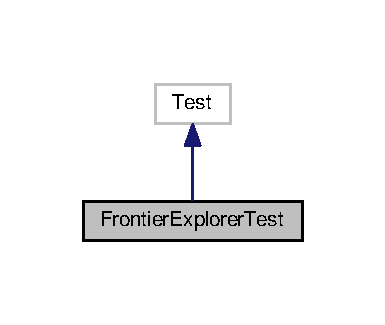
\includegraphics[width=185pt]{classFrontierExplorerTest__inherit__graph}
\end{center}
\end{figure}


Collaboration diagram for Frontier\+Explorer\+Test\+:
\nopagebreak
\begin{figure}[H]
\begin{center}
\leavevmode
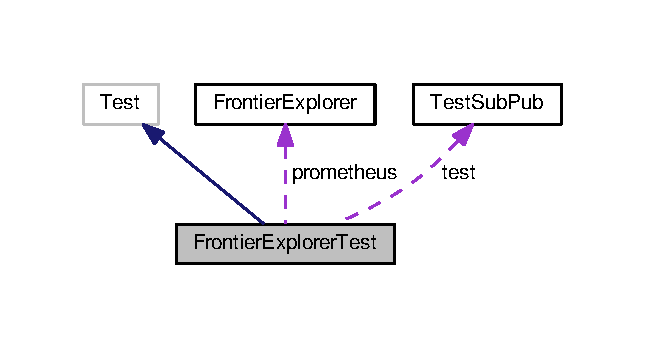
\includegraphics[width=310pt]{classFrontierExplorerTest__coll__graph}
\end{center}
\end{figure}
\subsection*{Public Member Functions}
\begin{DoxyCompactItemize}
\item 
void \hyperlink{classFrontierExplorerTest_a1471f30c1ded451b221c75dc7f8d18df}{Set\+Up} ()
\begin{DoxyCompactList}\small\item\em Setup Function used during tests. \end{DoxyCompactList}\item 
void \hyperlink{classFrontierExplorerTest_a7243e2b27064fbeedf27b65095a92e0a}{Tear\+Down} ()
\begin{DoxyCompactList}\small\item\em Teardown function used during tests. \end{DoxyCompactList}\end{DoxyCompactItemize}
\subsection*{Public Attributes}
\begin{DoxyCompactItemize}
\item 
ros\+::\+Node\+Handle {\bfseries nh}\hypertarget{classFrontierExplorerTest_a8c67a93eb7d215be22f24278e166ed69}{}\label{classFrontierExplorerTest_a8c67a93eb7d215be22f24278e166ed69}

\item 
\hyperlink{classFrontierExplorer}{Frontier\+Explorer} {\bfseries prometheus}\hypertarget{classFrontierExplorerTest_a0e28413e4df17dee970a008c6eaa13da}{}\label{classFrontierExplorerTest_a0e28413e4df17dee970a008c6eaa13da}

\item 
\hyperlink{classTestSubPub}{Test\+Sub\+Pub} {\bfseries test}\hypertarget{classFrontierExplorerTest_a52eef52386379d9353428c647af2cd98}{}\label{classFrontierExplorerTest_a52eef52386379d9353428c647af2cd98}

\end{DoxyCompactItemize}


\subsection{Detailed Description}
\hyperlink{classFrontierExplorerTest}{Frontier\+Explorer\+Test} Class. 

Test framework class for \hyperlink{classFrontierExplorer}{Frontier\+Explorer}. 

\subsection{Member Function Documentation}
\index{Frontier\+Explorer\+Test@{Frontier\+Explorer\+Test}!Set\+Up@{Set\+Up}}
\index{Set\+Up@{Set\+Up}!Frontier\+Explorer\+Test@{Frontier\+Explorer\+Test}}
\subsubsection[{\texorpdfstring{Set\+Up()}{SetUp()}}]{\setlength{\rightskip}{0pt plus 5cm}void Frontier\+Explorer\+Test\+::\+Set\+Up (
\begin{DoxyParamCaption}
{}
\end{DoxyParamCaption}
)\hspace{0.3cm}{\ttfamily [inline]}}\hypertarget{classFrontierExplorerTest_a1471f30c1ded451b221c75dc7f8d18df}{}\label{classFrontierExplorerTest_a1471f30c1ded451b221c75dc7f8d18df}


Setup Function used during tests. 


\begin{DoxyParams}{Parameters}
{\em none} & \\
\hline
\end{DoxyParams}
\begin{DoxyReturn}{Returns}
void 
\end{DoxyReturn}
\index{Frontier\+Explorer\+Test@{Frontier\+Explorer\+Test}!Tear\+Down@{Tear\+Down}}
\index{Tear\+Down@{Tear\+Down}!Frontier\+Explorer\+Test@{Frontier\+Explorer\+Test}}
\subsubsection[{\texorpdfstring{Tear\+Down()}{TearDown()}}]{\setlength{\rightskip}{0pt plus 5cm}void Frontier\+Explorer\+Test\+::\+Tear\+Down (
\begin{DoxyParamCaption}
{}
\end{DoxyParamCaption}
)\hspace{0.3cm}{\ttfamily [inline]}}\hypertarget{classFrontierExplorerTest_a7243e2b27064fbeedf27b65095a92e0a}{}\label{classFrontierExplorerTest_a7243e2b27064fbeedf27b65095a92e0a}


Teardown function used during tests. 


\begin{DoxyParams}{Parameters}
{\em none} & \\
\hline
\end{DoxyParams}
\begin{DoxyReturn}{Returns}
void 
\end{DoxyReturn}


The documentation for this class was generated from the following file\+:\begin{DoxyCompactItemize}
\item 
/home/hbk/\+Desktop/\+Software\+Development/\+Final\+Project/rosworld/src/prometheus\+\_\+frontier\+\_\+explorer/test/\hyperlink{FrontierExplorerTest_8cpp}{Frontier\+Explorer\+Test.\+cpp}\end{DoxyCompactItemize}

\hypertarget{classMap}{}\section{Map Class Reference}
\label{classMap}\index{Map@{Map}}


\hyperlink{classMap}{Map} Class.  




{\ttfamily \#include $<$Map.\+hpp$>$}

\subsection*{Public Member Functions}
\begin{DoxyCompactItemize}
\item 
\hyperlink{classMap_a0f5ad0fd4563497b4214038cbca8b582}{Map} ()
\begin{DoxyCompactList}\small\item\em Default constructor for \hyperlink{classMap}{Map} class. \end{DoxyCompactList}\item 
\hyperlink{classMap_aa403fbe09394ccf39747588f5168e3b2}{$\sim$\+Map} ()
\begin{DoxyCompactList}\small\item\em Destructor for \hyperlink{classMap}{Map} class. \end{DoxyCompactList}\item 
void \hyperlink{classMap_a5d91b013fec2766f7e7092a56829818b}{set\+Map\+Set} (bool value)
\begin{DoxyCompactList}\small\item\em Function to set flag for map initialized. \end{DoxyCompactList}\item 
bool \hyperlink{classMap_a360dfc995ca51cd427f4de531d95db17}{get\+Map\+Set} ()
\begin{DoxyCompactList}\small\item\em Function to get flag for map initialized. \end{DoxyCompactList}\item 
int \hyperlink{classMap_a92dda02fe42250c303e7fcfba73ba89b}{getmap\+Height} ()
\begin{DoxyCompactList}\small\item\em Function to get map height. \end{DoxyCompactList}\item 
int \hyperlink{classMap_a85aa3f85c7c57fffe6bcf6038b1ba288}{getmap\+Width} ()
\begin{DoxyCompactList}\small\item\em Function to get map width. \end{DoxyCompactList}\item 
double \hyperlink{classMap_a85211487535a00a6dd1cb003e2989238}{getmap\+Reso} ()
\begin{DoxyCompactList}\small\item\em Function to get map resolution. \end{DoxyCompactList}\item 
void \hyperlink{classMap_a0b24d829d0234c1422f89b873051a1a8}{setmap\+Height} (int value)
\begin{DoxyCompactList}\small\item\em Function to set map height. \end{DoxyCompactList}\item 
void \hyperlink{classMap_a9b2a2a242012e28deb30c323b42b8925}{setmap\+Width} (int value)
\begin{DoxyCompactList}\small\item\em Function to set map width. \end{DoxyCompactList}\item 
void \hyperlink{classMap_a65ddb9c03e089043bf819c1279a3f9f8}{setmap\+Reso} (double value)
\begin{DoxyCompactList}\small\item\em Function to set map resolution. \end{DoxyCompactList}\item 
void \hyperlink{classMap_a58b0c37d5d5e79dc1f23a0aa08536f6b}{set\+Origin} (geometry\+\_\+msgs\+::\+Point point)
\begin{DoxyCompactList}\small\item\em Function to set map origin. \end{DoxyCompactList}\item 
geometry\+\_\+msgs\+::\+Point \hyperlink{classMap_a471580c76f9da5202c5142bfb4ce6e2c}{get\+Origin} ()
\begin{DoxyCompactList}\small\item\em Function to get map origin. \end{DoxyCompactList}\item 
const std\+::vector$<$ std\+::vector$<$ \hyperlink{classMapNode}{Map\+Node} $>$ $>$ \& \hyperlink{classMap_ac7632edb702e1e9a62b3380e79a77825}{get\+Map} ()
\begin{DoxyCompactList}\small\item\em Function to get map. \end{DoxyCompactList}\item 
bool \hyperlink{classMap_aca7b17a488149e73990e12f6ec506f23}{update\+Map\+Params} (int current\+Width, int current\+Height, double current\+Reso, geometry\+\_\+msgs\+::\+Point map\+Center)
\begin{DoxyCompactList}\small\item\em Function to update map parameters. \end{DoxyCompactList}\item 
void \hyperlink{classMap_a4feacf5e0ca0961dc48dbdf7b7f42dd8}{update\+Map} (int current\+Width, int current\+Height, double current\+Reso, geometry\+\_\+msgs\+::\+Point map\+Center, const nav\+\_\+msgs\+::\+Occupancy\+Grid\+::\+Const\+Ptr \&msg)
\begin{DoxyCompactList}\small\item\em Function to update map. \end{DoxyCompactList}\item 
int \hyperlink{classMap_a707c9abbd2a2458c3fe885cf0d021906}{get\+Frontiers} ()
\begin{DoxyCompactList}\small\item\em Function to get frontiers from occupancy grid message. \end{DoxyCompactList}\item 
int \hyperlink{classMap_a18c425e2b087e715cb822af6ad8d99cc}{get\+Clusters} (int threshold)
\begin{DoxyCompactList}\small\item\em Function to make clusters from array of frontier location. \end{DoxyCompactList}\item 
std\+::vector$<$ std\+::pair$<$ double, double $>$ $>$ \hyperlink{classMap_ae2ff0d03880d709d140ed5b72166841b}{get\+Cluster\+Centroids} ()
\begin{DoxyCompactList}\small\item\em Function to calculate cluster centroids. \end{DoxyCompactList}\item 
const std\+::vector$<$ std\+::vector$<$ std\+::pair$<$ int, int $>$ $>$ $>$ \& \hyperlink{classMap_a4dc9d7e239d1bd24f2906331a4ef0cec}{get\+Frontier\+Cluster} ()
\begin{DoxyCompactList}\small\item\em Function to get cluster frontiers. \end{DoxyCompactList}\end{DoxyCompactItemize}


\subsection{Detailed Description}
\hyperlink{classMap}{Map} Class. 

Class for storing occupancy grid map 

\subsection{Constructor \& Destructor Documentation}
\index{Map@{Map}!Map@{Map}}
\index{Map@{Map}!Map@{Map}}
\subsubsection[{\texorpdfstring{Map()}{Map()}}]{\setlength{\rightskip}{0pt plus 5cm}Map\+::\+Map (
\begin{DoxyParamCaption}
{}
\end{DoxyParamCaption}
)}\hypertarget{classMap_a0f5ad0fd4563497b4214038cbca8b582}{}\label{classMap_a0f5ad0fd4563497b4214038cbca8b582}


Default constructor for \hyperlink{classMap}{Map} class. 


\begin{DoxyParams}{Parameters}
{\em none} & \\
\hline
\end{DoxyParams}
\begin{DoxyReturn}{Returns}
none 
\end{DoxyReturn}
\index{Map@{Map}!````~Map@{$\sim$\+Map}}
\index{````~Map@{$\sim$\+Map}!Map@{Map}}
\subsubsection[{\texorpdfstring{$\sim$\+Map()}{~Map()}}]{\setlength{\rightskip}{0pt plus 5cm}Map\+::$\sim$\+Map (
\begin{DoxyParamCaption}
{}
\end{DoxyParamCaption}
)}\hypertarget{classMap_aa403fbe09394ccf39747588f5168e3b2}{}\label{classMap_aa403fbe09394ccf39747588f5168e3b2}


Destructor for \hyperlink{classMap}{Map} class. 


\begin{DoxyParams}{Parameters}
{\em none} & \\
\hline
\end{DoxyParams}
\begin{DoxyReturn}{Returns}
none 
\end{DoxyReturn}


\subsection{Member Function Documentation}
\index{Map@{Map}!get\+Cluster\+Centroids@{get\+Cluster\+Centroids}}
\index{get\+Cluster\+Centroids@{get\+Cluster\+Centroids}!Map@{Map}}
\subsubsection[{\texorpdfstring{get\+Cluster\+Centroids()}{getClusterCentroids()}}]{\setlength{\rightskip}{0pt plus 5cm}std\+::vector$<$ std\+::pair$<$ double, double $>$ $>$ Map\+::get\+Cluster\+Centroids (
\begin{DoxyParamCaption}
{}
\end{DoxyParamCaption}
)}\hypertarget{classMap_ae2ff0d03880d709d140ed5b72166841b}{}\label{classMap_ae2ff0d03880d709d140ed5b72166841b}


Function to calculate cluster centroids. 


\begin{DoxyParams}{Parameters}
{\em none} & \\
\hline
\end{DoxyParams}
\begin{DoxyReturn}{Returns}
std\+::vector$<$std\+::pair$<$double, double$>$$>$ cluster centroid locations 
\end{DoxyReturn}
\index{Map@{Map}!get\+Clusters@{get\+Clusters}}
\index{get\+Clusters@{get\+Clusters}!Map@{Map}}
\subsubsection[{\texorpdfstring{get\+Clusters(int threshold)}{getClusters(int threshold)}}]{\setlength{\rightskip}{0pt plus 5cm}int Map\+::get\+Clusters (
\begin{DoxyParamCaption}
\item[{int}]{threshold}
\end{DoxyParamCaption}
)}\hypertarget{classMap_a18c425e2b087e715cb822af6ad8d99cc}{}\label{classMap_a18c425e2b087e715cb822af6ad8d99cc}


Function to make clusters from array of frontier location. 


\begin{DoxyParams}{Parameters}
{\em int} & threshold of frontiers to form cluster\\
\hline
\end{DoxyParams}
\begin{DoxyReturn}{Returns}
int number of clusters 
\end{DoxyReturn}
\index{Map@{Map}!get\+Frontier\+Cluster@{get\+Frontier\+Cluster}}
\index{get\+Frontier\+Cluster@{get\+Frontier\+Cluster}!Map@{Map}}
\subsubsection[{\texorpdfstring{get\+Frontier\+Cluster()}{getFrontierCluster()}}]{\setlength{\rightskip}{0pt plus 5cm}const std\+::vector$<$ std\+::vector$<$ std\+::pair$<$ int, int $>$ $>$ $>$ \& Map\+::get\+Frontier\+Cluster (
\begin{DoxyParamCaption}
{}
\end{DoxyParamCaption}
)}\hypertarget{classMap_a4dc9d7e239d1bd24f2906331a4ef0cec}{}\label{classMap_a4dc9d7e239d1bd24f2906331a4ef0cec}


Function to get cluster frontiers. 


\begin{DoxyParams}{Parameters}
{\em none} & \\
\hline
\end{DoxyParams}
\begin{DoxyReturn}{Returns}
std\+::vector$<$std\+::vector$<$std\+::pair$<$int, int$>$$>$$>$ cluster frontiers 
\end{DoxyReturn}
\index{Map@{Map}!get\+Frontiers@{get\+Frontiers}}
\index{get\+Frontiers@{get\+Frontiers}!Map@{Map}}
\subsubsection[{\texorpdfstring{get\+Frontiers()}{getFrontiers()}}]{\setlength{\rightskip}{0pt plus 5cm}int Map\+::get\+Frontiers (
\begin{DoxyParamCaption}
{}
\end{DoxyParamCaption}
)}\hypertarget{classMap_a707c9abbd2a2458c3fe885cf0d021906}{}\label{classMap_a707c9abbd2a2458c3fe885cf0d021906}


Function to get frontiers from occupancy grid message. 


\begin{DoxyParams}{Parameters}
{\em none} & \\
\hline
\end{DoxyParams}
\begin{DoxyReturn}{Returns}
int count of frontiers 
\end{DoxyReturn}
\index{Map@{Map}!get\+Map@{get\+Map}}
\index{get\+Map@{get\+Map}!Map@{Map}}
\subsubsection[{\texorpdfstring{get\+Map()}{getMap()}}]{\setlength{\rightskip}{0pt plus 5cm}const std\+::vector$<$ std\+::vector$<$ {\bf Map\+Node} $>$ $>$ \& Map\+::get\+Map (
\begin{DoxyParamCaption}
{}
\end{DoxyParamCaption}
)}\hypertarget{classMap_ac7632edb702e1e9a62b3380e79a77825}{}\label{classMap_ac7632edb702e1e9a62b3380e79a77825}


Function to get map. 


\begin{DoxyParams}{Parameters}
{\em none} & \\
\hline
\end{DoxyParams}
\begin{DoxyReturn}{Returns}
std\+::vector$<$std\+::vector$<$\+Map\+Node$>$$>$\& map 
\end{DoxyReturn}
\index{Map@{Map}!getmap\+Height@{getmap\+Height}}
\index{getmap\+Height@{getmap\+Height}!Map@{Map}}
\subsubsection[{\texorpdfstring{getmap\+Height()}{getmapHeight()}}]{\setlength{\rightskip}{0pt plus 5cm}int Map\+::getmap\+Height (
\begin{DoxyParamCaption}
{}
\end{DoxyParamCaption}
)}\hypertarget{classMap_a92dda02fe42250c303e7fcfba73ba89b}{}\label{classMap_a92dda02fe42250c303e7fcfba73ba89b}


Function to get map height. 


\begin{DoxyParams}{Parameters}
{\em none} & \\
\hline
\end{DoxyParams}
\begin{DoxyReturn}{Returns}
int map height 
\end{DoxyReturn}
\index{Map@{Map}!getmap\+Reso@{getmap\+Reso}}
\index{getmap\+Reso@{getmap\+Reso}!Map@{Map}}
\subsubsection[{\texorpdfstring{getmap\+Reso()}{getmapReso()}}]{\setlength{\rightskip}{0pt plus 5cm}double Map\+::getmap\+Reso (
\begin{DoxyParamCaption}
{}
\end{DoxyParamCaption}
)}\hypertarget{classMap_a85211487535a00a6dd1cb003e2989238}{}\label{classMap_a85211487535a00a6dd1cb003e2989238}


Function to get map resolution. 


\begin{DoxyParams}{Parameters}
{\em none} & \\
\hline
\end{DoxyParams}
\begin{DoxyReturn}{Returns}
double map resolution 
\end{DoxyReturn}
\index{Map@{Map}!get\+Map\+Set@{get\+Map\+Set}}
\index{get\+Map\+Set@{get\+Map\+Set}!Map@{Map}}
\subsubsection[{\texorpdfstring{get\+Map\+Set()}{getMapSet()}}]{\setlength{\rightskip}{0pt plus 5cm}bool Map\+::get\+Map\+Set (
\begin{DoxyParamCaption}
{}
\end{DoxyParamCaption}
)}\hypertarget{classMap_a360dfc995ca51cd427f4de531d95db17}{}\label{classMap_a360dfc995ca51cd427f4de531d95db17}


Function to get flag for map initialized. 


\begin{DoxyParams}{Parameters}
{\em none} & \\
\hline
\end{DoxyParams}
\begin{DoxyReturn}{Returns}
bool flag value to indicate initialized or not 
\end{DoxyReturn}
\index{Map@{Map}!getmap\+Width@{getmap\+Width}}
\index{getmap\+Width@{getmap\+Width}!Map@{Map}}
\subsubsection[{\texorpdfstring{getmap\+Width()}{getmapWidth()}}]{\setlength{\rightskip}{0pt plus 5cm}int Map\+::getmap\+Width (
\begin{DoxyParamCaption}
{}
\end{DoxyParamCaption}
)}\hypertarget{classMap_a85aa3f85c7c57fffe6bcf6038b1ba288}{}\label{classMap_a85aa3f85c7c57fffe6bcf6038b1ba288}


Function to get map width. 


\begin{DoxyParams}{Parameters}
{\em none} & \\
\hline
\end{DoxyParams}
\begin{DoxyReturn}{Returns}
int map width 
\end{DoxyReturn}
\index{Map@{Map}!get\+Origin@{get\+Origin}}
\index{get\+Origin@{get\+Origin}!Map@{Map}}
\subsubsection[{\texorpdfstring{get\+Origin()}{getOrigin()}}]{\setlength{\rightskip}{0pt plus 5cm}geometry\+\_\+msgs\+::\+Point Map\+::get\+Origin (
\begin{DoxyParamCaption}
{}
\end{DoxyParamCaption}
)}\hypertarget{classMap_a471580c76f9da5202c5142bfb4ce6e2c}{}\label{classMap_a471580c76f9da5202c5142bfb4ce6e2c}


Function to get map origin. 


\begin{DoxyParams}{Parameters}
{\em none} & \\
\hline
\end{DoxyParams}
\begin{DoxyReturn}{Returns}
geometry\+\_\+msgs\+::\+Point map origin 
\end{DoxyReturn}
\index{Map@{Map}!setmap\+Height@{setmap\+Height}}
\index{setmap\+Height@{setmap\+Height}!Map@{Map}}
\subsubsection[{\texorpdfstring{setmap\+Height(int value)}{setmapHeight(int value)}}]{\setlength{\rightskip}{0pt plus 5cm}void Map\+::setmap\+Height (
\begin{DoxyParamCaption}
\item[{int}]{value}
\end{DoxyParamCaption}
)}\hypertarget{classMap_a0b24d829d0234c1422f89b873051a1a8}{}\label{classMap_a0b24d829d0234c1422f89b873051a1a8}


Function to set map height. 


\begin{DoxyParams}{Parameters}
{\em int} & map height\\
\hline
\end{DoxyParams}
\begin{DoxyReturn}{Returns}
void 
\end{DoxyReturn}
\index{Map@{Map}!setmap\+Reso@{setmap\+Reso}}
\index{setmap\+Reso@{setmap\+Reso}!Map@{Map}}
\subsubsection[{\texorpdfstring{setmap\+Reso(double value)}{setmapReso(double value)}}]{\setlength{\rightskip}{0pt plus 5cm}void Map\+::setmap\+Reso (
\begin{DoxyParamCaption}
\item[{double}]{value}
\end{DoxyParamCaption}
)}\hypertarget{classMap_a65ddb9c03e089043bf819c1279a3f9f8}{}\label{classMap_a65ddb9c03e089043bf819c1279a3f9f8}


Function to set map resolution. 


\begin{DoxyParams}{Parameters}
{\em double} & map resolution\\
\hline
\end{DoxyParams}
\begin{DoxyReturn}{Returns}
void 
\end{DoxyReturn}
\index{Map@{Map}!set\+Map\+Set@{set\+Map\+Set}}
\index{set\+Map\+Set@{set\+Map\+Set}!Map@{Map}}
\subsubsection[{\texorpdfstring{set\+Map\+Set(bool value)}{setMapSet(bool value)}}]{\setlength{\rightskip}{0pt plus 5cm}void Map\+::set\+Map\+Set (
\begin{DoxyParamCaption}
\item[{bool}]{value}
\end{DoxyParamCaption}
)}\hypertarget{classMap_a5d91b013fec2766f7e7092a56829818b}{}\label{classMap_a5d91b013fec2766f7e7092a56829818b}


Function to set flag for map initialized. 


\begin{DoxyParams}{Parameters}
{\em bool} & flag value to indicate initialized or not\\
\hline
\end{DoxyParams}
\begin{DoxyReturn}{Returns}
void 
\end{DoxyReturn}
\index{Map@{Map}!setmap\+Width@{setmap\+Width}}
\index{setmap\+Width@{setmap\+Width}!Map@{Map}}
\subsubsection[{\texorpdfstring{setmap\+Width(int value)}{setmapWidth(int value)}}]{\setlength{\rightskip}{0pt plus 5cm}void Map\+::setmap\+Width (
\begin{DoxyParamCaption}
\item[{int}]{value}
\end{DoxyParamCaption}
)}\hypertarget{classMap_a9b2a2a242012e28deb30c323b42b8925}{}\label{classMap_a9b2a2a242012e28deb30c323b42b8925}


Function to set map width. 


\begin{DoxyParams}{Parameters}
{\em int} & map width\\
\hline
\end{DoxyParams}
\begin{DoxyReturn}{Returns}
void 
\end{DoxyReturn}
\index{Map@{Map}!set\+Origin@{set\+Origin}}
\index{set\+Origin@{set\+Origin}!Map@{Map}}
\subsubsection[{\texorpdfstring{set\+Origin(geometry\+\_\+msgs\+::\+Point point)}{setOrigin(geometry_msgs::Point point)}}]{\setlength{\rightskip}{0pt plus 5cm}void Map\+::set\+Origin (
\begin{DoxyParamCaption}
\item[{geometry\+\_\+msgs\+::\+Point}]{point}
\end{DoxyParamCaption}
)}\hypertarget{classMap_a58b0c37d5d5e79dc1f23a0aa08536f6b}{}\label{classMap_a58b0c37d5d5e79dc1f23a0aa08536f6b}


Function to set map origin. 


\begin{DoxyParams}{Parameters}
{\em geometry\+\_\+msgs\+::\+Point} & map origin\\
\hline
\end{DoxyParams}
\begin{DoxyReturn}{Returns}
void 
\end{DoxyReturn}
\index{Map@{Map}!update\+Map@{update\+Map}}
\index{update\+Map@{update\+Map}!Map@{Map}}
\subsubsection[{\texorpdfstring{update\+Map(int current\+Width, int current\+Height, double current\+Reso, geometry\+\_\+msgs\+::\+Point map\+Center, const nav\+\_\+msgs\+::\+Occupancy\+Grid\+::\+Const\+Ptr \&msg)}{updateMap(int currentWidth, int currentHeight, double currentReso, geometry_msgs::Point mapCenter, const nav_msgs::OccupancyGrid::ConstPtr &msg)}}]{\setlength{\rightskip}{0pt plus 5cm}void Map\+::update\+Map (
\begin{DoxyParamCaption}
\item[{int}]{current\+Width, }
\item[{int}]{current\+Height, }
\item[{double}]{current\+Reso, }
\item[{geometry\+\_\+msgs\+::\+Point}]{map\+Center, }
\item[{const nav\+\_\+msgs\+::\+Occupancy\+Grid\+::\+Const\+Ptr \&}]{msg}
\end{DoxyParamCaption}
)}\hypertarget{classMap_a4feacf5e0ca0961dc48dbdf7b7f42dd8}{}\label{classMap_a4feacf5e0ca0961dc48dbdf7b7f42dd8}


Function to update map. 


\begin{DoxyParams}{Parameters}
{\em int} & map width \\
\hline
{\em int} & map height \\
\hline
{\em double} & map resolution \\
\hline
{\em geometry\+\_\+msgs\+::\+Point} & map center/origin \\
\hline
{\em nav\+\_\+msgs\+::\+Occupancy\+Grid\+::\+Const\+Ptr\&} & occupancy grid map message\\
\hline
\end{DoxyParams}
\begin{DoxyReturn}{Returns}
bool update status 
\end{DoxyReturn}
\index{Map@{Map}!update\+Map\+Params@{update\+Map\+Params}}
\index{update\+Map\+Params@{update\+Map\+Params}!Map@{Map}}
\subsubsection[{\texorpdfstring{update\+Map\+Params(int current\+Width, int current\+Height, double current\+Reso, geometry\+\_\+msgs\+::\+Point map\+Center)}{updateMapParams(int currentWidth, int currentHeight, double currentReso, geometry_msgs::Point mapCenter)}}]{\setlength{\rightskip}{0pt plus 5cm}bool Map\+::update\+Map\+Params (
\begin{DoxyParamCaption}
\item[{int}]{current\+Width, }
\item[{int}]{current\+Height, }
\item[{double}]{current\+Reso, }
\item[{geometry\+\_\+msgs\+::\+Point}]{map\+Center}
\end{DoxyParamCaption}
)}\hypertarget{classMap_aca7b17a488149e73990e12f6ec506f23}{}\label{classMap_aca7b17a488149e73990e12f6ec506f23}


Function to update map parameters. 


\begin{DoxyParams}{Parameters}
{\em int} & map width \\
\hline
{\em int} & map height \\
\hline
{\em double} & map resolution \\
\hline
{\em geometry\+\_\+msgs\+::\+Point} & map center/origin\\
\hline
\end{DoxyParams}
\begin{DoxyReturn}{Returns}
bool update status 
\end{DoxyReturn}


The documentation for this class was generated from the following files\+:\begin{DoxyCompactItemize}
\item 
/home/hbk/\+Desktop/\+Software\+Development/\+Final\+Project/rosworld/src/prometheus\+\_\+frontier\+\_\+explorer/include/\hyperlink{Map_8hpp}{Map.\+hpp}\item 
/home/hbk/\+Desktop/\+Software\+Development/\+Final\+Project/rosworld/src/prometheus\+\_\+frontier\+\_\+explorer/src/\hyperlink{Map_8cpp}{Map.\+cpp}\end{DoxyCompactItemize}

\hypertarget{classMapNode}{}\section{Map\+Node Class Reference}
\label{classMapNode}\index{Map\+Node@{Map\+Node}}


\hyperlink{classMapNode}{Map\+Node} Class.  




{\ttfamily \#include $<$Map\+Node.\+hpp$>$}

\subsection*{Public Member Functions}
\begin{DoxyCompactItemize}
\item 
\hyperlink{classMapNode_aa4e1fb66b032e08781093ffb7fe03885}{Map\+Node} ()
\begin{DoxyCompactList}\small\item\em Default constructor for \hyperlink{classMapNode}{Map\+Node} class. \end{DoxyCompactList}\item 
\hyperlink{classMapNode_a380098b662362882a2d5ca3bd5004fc1}{$\sim$\+Map\+Node} ()
\begin{DoxyCompactList}\small\item\em Destructor for \hyperlink{classMapNode}{Map\+Node} class. \end{DoxyCompactList}\item 
float \hyperlink{classMapNode_a2049f6ba89f765acde265d0f381a0e2c}{getX} ()
\begin{DoxyCompactList}\small\item\em Function to get x-\/coordinate for map node. \end{DoxyCompactList}\item 
float \hyperlink{classMapNode_a05b7f28bfdbb7ae2def6a710a3c68b13}{getY} ()
\begin{DoxyCompactList}\small\item\em Function to get y-\/coordinate for map node. \end{DoxyCompactList}\item 
int8\+\_\+t \hyperlink{classMapNode_a429349451143f622dce0fdcc77b8cbb8}{get\+Probability} ()
\begin{DoxyCompactList}\small\item\em Function to get probability for map node. \end{DoxyCompactList}\item 
void \hyperlink{classMapNode_a3e8c9e037ee794230866d86d06a74f04}{setX} (float value)
\begin{DoxyCompactList}\small\item\em Function to set x-\/coordinate for map node. \end{DoxyCompactList}\item 
void \hyperlink{classMapNode_a4b5be155789e2f163a50c983f209dd3d}{setY} (float value)
\begin{DoxyCompactList}\small\item\em Function to set y-\/coordinate for map node. \end{DoxyCompactList}\item 
void \hyperlink{classMapNode_a1afc2f93a9a43f8455e1aad31e558d60}{set\+Probability} (int8\+\_\+t value)
\begin{DoxyCompactList}\small\item\em Function to set probability for map node. \end{DoxyCompactList}\item 
bool \hyperlink{classMapNode_a1fe4585ed4d0b47f7f243c55d7696a84}{getis\+Frontier} ()
\begin{DoxyCompactList}\small\item\em Function to get isfrontier flag for map node. \end{DoxyCompactList}\item 
void \hyperlink{classMapNode_a9d29e10437231fb65dedffdcb855be66}{setis\+Frontier} (bool value)
\begin{DoxyCompactList}\small\item\em Function to set isfrontier flag for map node. \end{DoxyCompactList}\item 
int \hyperlink{classMapNode_a238c0b6630846662b2ad9c34c242af5d}{get\+Frontier\+Index} ()
\begin{DoxyCompactList}\small\item\em Function to get frontier index flag for map node. \end{DoxyCompactList}\item 
void \hyperlink{classMapNode_a859724964cd0718994819500ba482079}{set\+Frontier\+Index} (int value)
\begin{DoxyCompactList}\small\item\em Function to set frontier index flag for map node. \end{DoxyCompactList}\end{DoxyCompactItemize}


\subsection{Detailed Description}
\hyperlink{classMapNode}{Map\+Node} Class. 

Class for storing occupancy grid map nodes 

\subsection{Constructor \& Destructor Documentation}
\index{Map\+Node@{Map\+Node}!Map\+Node@{Map\+Node}}
\index{Map\+Node@{Map\+Node}!Map\+Node@{Map\+Node}}
\subsubsection[{\texorpdfstring{Map\+Node()}{MapNode()}}]{\setlength{\rightskip}{0pt plus 5cm}Map\+Node\+::\+Map\+Node (
\begin{DoxyParamCaption}
{}
\end{DoxyParamCaption}
)}\hypertarget{classMapNode_aa4e1fb66b032e08781093ffb7fe03885}{}\label{classMapNode_aa4e1fb66b032e08781093ffb7fe03885}


Default constructor for \hyperlink{classMapNode}{Map\+Node} class. 


\begin{DoxyParams}{Parameters}
{\em none} & \\
\hline
\end{DoxyParams}
\begin{DoxyReturn}{Returns}
none 
\end{DoxyReturn}
\index{Map\+Node@{Map\+Node}!````~Map\+Node@{$\sim$\+Map\+Node}}
\index{````~Map\+Node@{$\sim$\+Map\+Node}!Map\+Node@{Map\+Node}}
\subsubsection[{\texorpdfstring{$\sim$\+Map\+Node()}{~MapNode()}}]{\setlength{\rightskip}{0pt plus 5cm}Map\+Node\+::$\sim$\+Map\+Node (
\begin{DoxyParamCaption}
{}
\end{DoxyParamCaption}
)}\hypertarget{classMapNode_a380098b662362882a2d5ca3bd5004fc1}{}\label{classMapNode_a380098b662362882a2d5ca3bd5004fc1}


Destructor for \hyperlink{classMapNode}{Map\+Node} class. 


\begin{DoxyParams}{Parameters}
{\em none} & \\
\hline
\end{DoxyParams}
\begin{DoxyReturn}{Returns}
none 
\end{DoxyReturn}


\subsection{Member Function Documentation}
\index{Map\+Node@{Map\+Node}!get\+Frontier\+Index@{get\+Frontier\+Index}}
\index{get\+Frontier\+Index@{get\+Frontier\+Index}!Map\+Node@{Map\+Node}}
\subsubsection[{\texorpdfstring{get\+Frontier\+Index()}{getFrontierIndex()}}]{\setlength{\rightskip}{0pt plus 5cm}int Map\+Node\+::get\+Frontier\+Index (
\begin{DoxyParamCaption}
{}
\end{DoxyParamCaption}
)}\hypertarget{classMapNode_a238c0b6630846662b2ad9c34c242af5d}{}\label{classMapNode_a238c0b6630846662b2ad9c34c242af5d}


Function to get frontier index flag for map node. 


\begin{DoxyParams}{Parameters}
{\em none} & \\
\hline
\end{DoxyParams}
\begin{DoxyReturn}{Returns}
int frontier index 
\end{DoxyReturn}
\index{Map\+Node@{Map\+Node}!getis\+Frontier@{getis\+Frontier}}
\index{getis\+Frontier@{getis\+Frontier}!Map\+Node@{Map\+Node}}
\subsubsection[{\texorpdfstring{getis\+Frontier()}{getisFrontier()}}]{\setlength{\rightskip}{0pt plus 5cm}bool Map\+Node\+::getis\+Frontier (
\begin{DoxyParamCaption}
{}
\end{DoxyParamCaption}
)}\hypertarget{classMapNode_a1fe4585ed4d0b47f7f243c55d7696a84}{}\label{classMapNode_a1fe4585ed4d0b47f7f243c55d7696a84}


Function to get isfrontier flag for map node. 


\begin{DoxyParams}{Parameters}
{\em none} & \\
\hline
\end{DoxyParams}
\begin{DoxyReturn}{Returns}
bool isfrontier flag 
\end{DoxyReturn}
\index{Map\+Node@{Map\+Node}!get\+Probability@{get\+Probability}}
\index{get\+Probability@{get\+Probability}!Map\+Node@{Map\+Node}}
\subsubsection[{\texorpdfstring{get\+Probability()}{getProbability()}}]{\setlength{\rightskip}{0pt plus 5cm}int8\+\_\+t Map\+Node\+::get\+Probability (
\begin{DoxyParamCaption}
{}
\end{DoxyParamCaption}
)}\hypertarget{classMapNode_a429349451143f622dce0fdcc77b8cbb8}{}\label{classMapNode_a429349451143f622dce0fdcc77b8cbb8}


Function to get probability for map node. 


\begin{DoxyParams}{Parameters}
{\em none} & \\
\hline
\end{DoxyParams}
\begin{DoxyReturn}{Returns}
int8\+\_\+t probability of node 
\end{DoxyReturn}
\index{Map\+Node@{Map\+Node}!getX@{getX}}
\index{getX@{getX}!Map\+Node@{Map\+Node}}
\subsubsection[{\texorpdfstring{get\+X()}{getX()}}]{\setlength{\rightskip}{0pt plus 5cm}float Map\+Node\+::getX (
\begin{DoxyParamCaption}
{}
\end{DoxyParamCaption}
)}\hypertarget{classMapNode_a2049f6ba89f765acde265d0f381a0e2c}{}\label{classMapNode_a2049f6ba89f765acde265d0f381a0e2c}


Function to get x-\/coordinate for map node. 


\begin{DoxyParams}{Parameters}
{\em none} & \\
\hline
\end{DoxyParams}
\begin{DoxyReturn}{Returns}
float x-\/coordinate of node 
\end{DoxyReturn}
\index{Map\+Node@{Map\+Node}!getY@{getY}}
\index{getY@{getY}!Map\+Node@{Map\+Node}}
\subsubsection[{\texorpdfstring{get\+Y()}{getY()}}]{\setlength{\rightskip}{0pt plus 5cm}float Map\+Node\+::getY (
\begin{DoxyParamCaption}
{}
\end{DoxyParamCaption}
)}\hypertarget{classMapNode_a05b7f28bfdbb7ae2def6a710a3c68b13}{}\label{classMapNode_a05b7f28bfdbb7ae2def6a710a3c68b13}


Function to get y-\/coordinate for map node. 


\begin{DoxyParams}{Parameters}
{\em none} & \\
\hline
\end{DoxyParams}
\begin{DoxyReturn}{Returns}
float y-\/coordinate of node 
\end{DoxyReturn}
\index{Map\+Node@{Map\+Node}!set\+Frontier\+Index@{set\+Frontier\+Index}}
\index{set\+Frontier\+Index@{set\+Frontier\+Index}!Map\+Node@{Map\+Node}}
\subsubsection[{\texorpdfstring{set\+Frontier\+Index(int value)}{setFrontierIndex(int value)}}]{\setlength{\rightskip}{0pt plus 5cm}void Map\+Node\+::set\+Frontier\+Index (
\begin{DoxyParamCaption}
\item[{int}]{value}
\end{DoxyParamCaption}
)}\hypertarget{classMapNode_a859724964cd0718994819500ba482079}{}\label{classMapNode_a859724964cd0718994819500ba482079}


Function to set frontier index flag for map node. 


\begin{DoxyParams}{Parameters}
{\em int} & frontier index\\
\hline
\end{DoxyParams}
\begin{DoxyReturn}{Returns}
void 
\end{DoxyReturn}
\index{Map\+Node@{Map\+Node}!setis\+Frontier@{setis\+Frontier}}
\index{setis\+Frontier@{setis\+Frontier}!Map\+Node@{Map\+Node}}
\subsubsection[{\texorpdfstring{setis\+Frontier(bool value)}{setisFrontier(bool value)}}]{\setlength{\rightskip}{0pt plus 5cm}void Map\+Node\+::setis\+Frontier (
\begin{DoxyParamCaption}
\item[{bool}]{value}
\end{DoxyParamCaption}
)}\hypertarget{classMapNode_a9d29e10437231fb65dedffdcb855be66}{}\label{classMapNode_a9d29e10437231fb65dedffdcb855be66}


Function to set isfrontier flag for map node. 


\begin{DoxyParams}{Parameters}
{\em bool} & isfrontier flag\\
\hline
\end{DoxyParams}
\begin{DoxyReturn}{Returns}
void 
\end{DoxyReturn}
\index{Map\+Node@{Map\+Node}!set\+Probability@{set\+Probability}}
\index{set\+Probability@{set\+Probability}!Map\+Node@{Map\+Node}}
\subsubsection[{\texorpdfstring{set\+Probability(int8\+\_\+t value)}{setProbability(int8_t value)}}]{\setlength{\rightskip}{0pt plus 5cm}void Map\+Node\+::set\+Probability (
\begin{DoxyParamCaption}
\item[{int8\+\_\+t}]{value}
\end{DoxyParamCaption}
)}\hypertarget{classMapNode_a1afc2f93a9a43f8455e1aad31e558d60}{}\label{classMapNode_a1afc2f93a9a43f8455e1aad31e558d60}


Function to set probability for map node. 


\begin{DoxyParams}{Parameters}
{\em int8\+\_\+t} & probability of node\\
\hline
\end{DoxyParams}
\begin{DoxyReturn}{Returns}
voide 
\end{DoxyReturn}
\index{Map\+Node@{Map\+Node}!setX@{setX}}
\index{setX@{setX}!Map\+Node@{Map\+Node}}
\subsubsection[{\texorpdfstring{set\+X(float value)}{setX(float value)}}]{\setlength{\rightskip}{0pt plus 5cm}void Map\+Node\+::setX (
\begin{DoxyParamCaption}
\item[{float}]{value}
\end{DoxyParamCaption}
)}\hypertarget{classMapNode_a3e8c9e037ee794230866d86d06a74f04}{}\label{classMapNode_a3e8c9e037ee794230866d86d06a74f04}


Function to set x-\/coordinate for map node. 


\begin{DoxyParams}{Parameters}
{\em float} & x-\/coordinate of node\\
\hline
\end{DoxyParams}
\begin{DoxyReturn}{Returns}
void 
\end{DoxyReturn}
\index{Map\+Node@{Map\+Node}!setY@{setY}}
\index{setY@{setY}!Map\+Node@{Map\+Node}}
\subsubsection[{\texorpdfstring{set\+Y(float value)}{setY(float value)}}]{\setlength{\rightskip}{0pt plus 5cm}void Map\+Node\+::setY (
\begin{DoxyParamCaption}
\item[{float}]{value}
\end{DoxyParamCaption}
)}\hypertarget{classMapNode_a4b5be155789e2f163a50c983f209dd3d}{}\label{classMapNode_a4b5be155789e2f163a50c983f209dd3d}


Function to set y-\/coordinate for map node. 


\begin{DoxyParams}{Parameters}
{\em float} & y-\/coordinate of node\\
\hline
\end{DoxyParams}
\begin{DoxyReturn}{Returns}
void 
\end{DoxyReturn}


The documentation for this class was generated from the following files\+:\begin{DoxyCompactItemize}
\item 
/home/hbk/\+Desktop/\+Software\+Development/\+Final\+Project/rosworld/src/prometheus\+\_\+frontier\+\_\+explorer/include/\hyperlink{MapNode_8hpp}{Map\+Node.\+hpp}\item 
/home/hbk/\+Desktop/\+Software\+Development/\+Final\+Project/rosworld/src/prometheus\+\_\+frontier\+\_\+explorer/src/\hyperlink{MapNode_8cpp}{Map\+Node.\+cpp}\end{DoxyCompactItemize}

\hypertarget{classMapNodeTest}{}\section{Map\+Node\+Test Class Reference}
\label{classMapNodeTest}\index{Map\+Node\+Test@{Map\+Node\+Test}}


\hyperlink{classMapNodeTest}{Map\+Node\+Test} Class.  




Inheritance diagram for Map\+Node\+Test\+:
\nopagebreak
\begin{figure}[H]
\begin{center}
\leavevmode
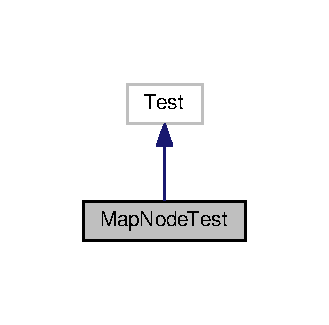
\includegraphics[width=158pt]{classMapNodeTest__inherit__graph}
\end{center}
\end{figure}


Collaboration diagram for Map\+Node\+Test\+:
\nopagebreak
\begin{figure}[H]
\begin{center}
\leavevmode
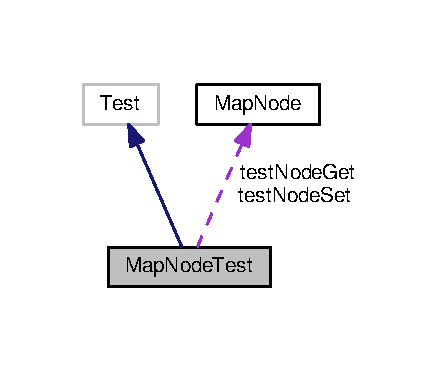
\includegraphics[width=211pt]{classMapNodeTest__coll__graph}
\end{center}
\end{figure}
\subsection*{Public Member Functions}
\begin{DoxyCompactItemize}
\item 
void \hyperlink{classMapNodeTest_a932784523d427c895556b50866646add}{Set\+Up} ()
\begin{DoxyCompactList}\small\item\em Setup Function used during tests. \end{DoxyCompactList}\item 
void \hyperlink{classMapNodeTest_a5367ace6e713049e58f596a6488a4570}{Tear\+Down} ()
\begin{DoxyCompactList}\small\item\em Teardown function used during tests. \end{DoxyCompactList}\end{DoxyCompactItemize}
\subsection*{Public Attributes}
\begin{DoxyCompactItemize}
\item 
\hyperlink{classMapNode}{Map\+Node} {\bfseries test\+Node\+Set}\hypertarget{classMapNodeTest_a2f493683755b45e53f25a97e628ebb03}{}\label{classMapNodeTest_a2f493683755b45e53f25a97e628ebb03}

\item 
\hyperlink{classMapNode}{Map\+Node} {\bfseries test\+Node\+Get}\hypertarget{classMapNodeTest_a5a9e610742272157ad94a7a439dc079d}{}\label{classMapNodeTest_a5a9e610742272157ad94a7a439dc079d}

\item 
float {\bfseries x}\hypertarget{classMapNodeTest_ade7b439cf615d750e8f4ad5a977e2938}{}\label{classMapNodeTest_ade7b439cf615d750e8f4ad5a977e2938}

\item 
float {\bfseries y}\hypertarget{classMapNodeTest_ad6ae973ba822364cc90756f73015ba4a}{}\label{classMapNodeTest_ad6ae973ba822364cc90756f73015ba4a}

\item 
int8\+\_\+t {\bfseries prob}\hypertarget{classMapNodeTest_a6f4c4344863c169a9b733eb357c8ec2a}{}\label{classMapNodeTest_a6f4c4344863c169a9b733eb357c8ec2a}

\item 
bool {\bfseries frontier\+Flag}\hypertarget{classMapNodeTest_afd3c21a4c35476863aa06c477a86bcb3}{}\label{classMapNodeTest_afd3c21a4c35476863aa06c477a86bcb3}

\item 
int {\bfseries frontier\+Index}\hypertarget{classMapNodeTest_aa57879f8f1138116b711426f86709469}{}\label{classMapNodeTest_aa57879f8f1138116b711426f86709469}

\end{DoxyCompactItemize}


\subsection{Detailed Description}
\hyperlink{classMapNodeTest}{Map\+Node\+Test} Class. 

Test framework class for \hyperlink{classMapNodeTest}{Map\+Node\+Test}. 

\subsection{Member Function Documentation}
\index{Map\+Node\+Test@{Map\+Node\+Test}!Set\+Up@{Set\+Up}}
\index{Set\+Up@{Set\+Up}!Map\+Node\+Test@{Map\+Node\+Test}}
\subsubsection[{\texorpdfstring{Set\+Up()}{SetUp()}}]{\setlength{\rightskip}{0pt plus 5cm}void Map\+Node\+Test\+::\+Set\+Up (
\begin{DoxyParamCaption}
{}
\end{DoxyParamCaption}
)\hspace{0.3cm}{\ttfamily [inline]}}\hypertarget{classMapNodeTest_a932784523d427c895556b50866646add}{}\label{classMapNodeTest_a932784523d427c895556b50866646add}


Setup Function used during tests. 


\begin{DoxyParams}{Parameters}
{\em none} & \\
\hline
\end{DoxyParams}
\begin{DoxyReturn}{Returns}
void 
\end{DoxyReturn}
\index{Map\+Node\+Test@{Map\+Node\+Test}!Tear\+Down@{Tear\+Down}}
\index{Tear\+Down@{Tear\+Down}!Map\+Node\+Test@{Map\+Node\+Test}}
\subsubsection[{\texorpdfstring{Tear\+Down()}{TearDown()}}]{\setlength{\rightskip}{0pt plus 5cm}void Map\+Node\+Test\+::\+Tear\+Down (
\begin{DoxyParamCaption}
{}
\end{DoxyParamCaption}
)\hspace{0.3cm}{\ttfamily [inline]}}\hypertarget{classMapNodeTest_a5367ace6e713049e58f596a6488a4570}{}\label{classMapNodeTest_a5367ace6e713049e58f596a6488a4570}


Teardown function used during tests. 


\begin{DoxyParams}{Parameters}
{\em none} & \\
\hline
\end{DoxyParams}
\begin{DoxyReturn}{Returns}
void 
\end{DoxyReturn}


The documentation for this class was generated from the following file\+:\begin{DoxyCompactItemize}
\item 
/home/hbk/\+Desktop/\+Software\+Development/\+Final\+Project/rosworld/src/prometheus\+\_\+frontier\+\_\+explorer/test/\hyperlink{MapNodeTest_8cpp}{Map\+Node\+Test.\+cpp}\end{DoxyCompactItemize}

\hypertarget{classMapTest}{}\section{Map\+Test Class Reference}
\label{classMapTest}\index{Map\+Test@{Map\+Test}}


\hyperlink{classMapTest}{Map\+Test} Class.  




Inheritance diagram for Map\+Test\+:
\nopagebreak
\begin{figure}[H]
\begin{center}
\leavevmode
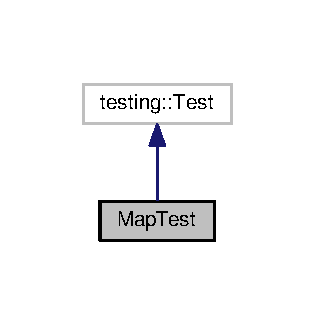
\includegraphics[width=151pt]{classMapTest__inherit__graph}
\end{center}
\end{figure}


Collaboration diagram for Map\+Test\+:
\nopagebreak
\begin{figure}[H]
\begin{center}
\leavevmode
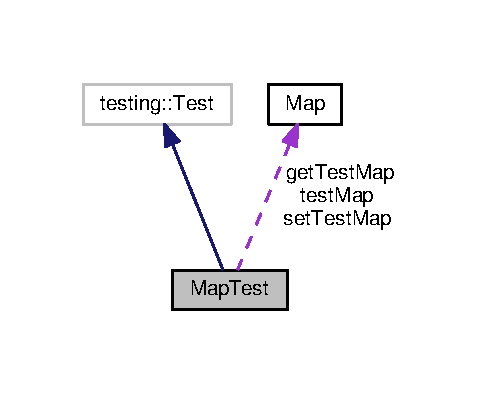
\includegraphics[width=230pt]{classMapTest__coll__graph}
\end{center}
\end{figure}
\subsection*{Public Member Functions}
\begin{DoxyCompactItemize}
\item 
void \hyperlink{classMapTest_a24e2117680abf39f0a8c87c7fffa45fd}{Set\+Up} ()
\begin{DoxyCompactList}\small\item\em Setup Function used during tests. \end{DoxyCompactList}\item 
void \hyperlink{classMapTest_a4114fafbb5db18eb0052123d062ba18a}{Tear\+Down} ()
\begin{DoxyCompactList}\small\item\em Teardown function used during tests. \end{DoxyCompactList}\end{DoxyCompactItemize}
\subsection*{Public Attributes}
\begin{DoxyCompactItemize}
\item 
nav\+\_\+msgs\+::\+Map\+Meta\+Data {\bfseries info}\hypertarget{classMapTest_a333b326a68d2b79700fcddb47b7f57e6}{}\label{classMapTest_a333b326a68d2b79700fcddb47b7f57e6}

\item 
\hyperlink{classMap}{Map} {\bfseries test\+Map}\hypertarget{classMapTest_aff93358464beda2ebc07e8a8ba4eea08}{}\label{classMapTest_aff93358464beda2ebc07e8a8ba4eea08}

\item 
\hyperlink{classMap}{Map} {\bfseries set\+Test\+Map}\hypertarget{classMapTest_a36961e285b2985e36e1e7a461c8d4ec1}{}\label{classMapTest_a36961e285b2985e36e1e7a461c8d4ec1}

\item 
\hyperlink{classMap}{Map} {\bfseries get\+Test\+Map}\hypertarget{classMapTest_a5d4095ff258b0e05bf5ac635f9876dbb}{}\label{classMapTest_a5d4095ff258b0e05bf5ac635f9876dbb}

\item 
bool {\bfseries map\+Flag}\hypertarget{classMapTest_a496078ef68b6350c22d01e8feef78ddf}{}\label{classMapTest_a496078ef68b6350c22d01e8feef78ddf}

\item 
int {\bfseries width\+Test}\hypertarget{classMapTest_aea4202c465fdd1e3e43973254d0ced2b}{}\label{classMapTest_aea4202c465fdd1e3e43973254d0ced2b}

\item 
int {\bfseries height\+Test}\hypertarget{classMapTest_a8f2c13fd53b8f7bf8d37ac6e20e2bcb6}{}\label{classMapTest_a8f2c13fd53b8f7bf8d37ac6e20e2bcb6}

\item 
float {\bfseries reso\+Test}\hypertarget{classMapTest_a84ae73719f2d147a7251d6d643962b97}{}\label{classMapTest_a84ae73719f2d147a7251d6d643962b97}

\item 
geometry\+\_\+msgs\+::\+Point {\bfseries currcentertest}\hypertarget{classMapTest_a8fd0be31559213669a0664bdfd73bc85}{}\label{classMapTest_a8fd0be31559213669a0664bdfd73bc85}

\end{DoxyCompactItemize}


\subsection{Detailed Description}
\hyperlink{classMapTest}{Map\+Test} Class. 

Test framework class for \hyperlink{classMapTest}{Map\+Test}. 

\subsection{Member Function Documentation}
\index{Map\+Test@{Map\+Test}!Set\+Up@{Set\+Up}}
\index{Set\+Up@{Set\+Up}!Map\+Test@{Map\+Test}}
\subsubsection[{\texorpdfstring{Set\+Up()}{SetUp()}}]{\setlength{\rightskip}{0pt plus 5cm}void Map\+Test\+::\+Set\+Up (
\begin{DoxyParamCaption}
{}
\end{DoxyParamCaption}
)\hspace{0.3cm}{\ttfamily [inline]}}\hypertarget{classMapTest_a24e2117680abf39f0a8c87c7fffa45fd}{}\label{classMapTest_a24e2117680abf39f0a8c87c7fffa45fd}


Setup Function used during tests. 


\begin{DoxyParams}{Parameters}
{\em none} & \\
\hline
\end{DoxyParams}
\begin{DoxyReturn}{Returns}
void 
\end{DoxyReturn}
\index{Map\+Test@{Map\+Test}!Tear\+Down@{Tear\+Down}}
\index{Tear\+Down@{Tear\+Down}!Map\+Test@{Map\+Test}}
\subsubsection[{\texorpdfstring{Tear\+Down()}{TearDown()}}]{\setlength{\rightskip}{0pt plus 5cm}void Map\+Test\+::\+Tear\+Down (
\begin{DoxyParamCaption}
{}
\end{DoxyParamCaption}
)\hspace{0.3cm}{\ttfamily [inline]}}\hypertarget{classMapTest_a4114fafbb5db18eb0052123d062ba18a}{}\label{classMapTest_a4114fafbb5db18eb0052123d062ba18a}


Teardown function used during tests. 


\begin{DoxyParams}{Parameters}
{\em none} & \\
\hline
\end{DoxyParams}
\begin{DoxyReturn}{Returns}
void 
\end{DoxyReturn}


The documentation for this class was generated from the following file\+:\begin{DoxyCompactItemize}
\item 
/home/hbk/\+Desktop/\+Software\+Development/\+Final\+Project/rosworld/src/prometheus\+\_\+frontier\+\_\+explorer/test/\hyperlink{MapTest_8cpp}{Map\+Test.\+cpp}\end{DoxyCompactItemize}

\hypertarget{classTestSubPub}{}\section{Test\+Sub\+Pub Class Reference}
\label{classTestSubPub}\index{Test\+Sub\+Pub@{Test\+Sub\+Pub}}


\hyperlink{classTestSubPub}{Test\+Sub\+Pub} Class.  


\subsection*{Public Member Functions}
\begin{DoxyCompactItemize}
\item 
void {\bfseries test\+Marker\+Publish} (const visualization\+\_\+msgs\+::\+Marker\+Array\+::\+Const\+Ptr \&msg)\hypertarget{classTestSubPub_aa6c1d296085874a313c62ee6c7c4f8ce}{}\label{classTestSubPub_aa6c1d296085874a313c62ee6c7c4f8ce}

\item 
void {\bfseries test\+Velocity\+Publish} (const geometry\+\_\+msgs\+::\+Twist\+::\+Const\+Ptr \&msg)\hypertarget{classTestSubPub_a854cfe325476ea421a169615ce12fce1}{}\label{classTestSubPub_a854cfe325476ea421a169615ce12fce1}

\end{DoxyCompactItemize}


\subsection{Detailed Description}
\hyperlink{classTestSubPub}{Test\+Sub\+Pub} Class. 

Test class for publisher and subscriber test. 

The documentation for this class was generated from the following file\+:\begin{DoxyCompactItemize}
\item 
/home/hbk/\+Desktop/\+Software\+Development/\+Final\+Project/rosworld/src/prometheus\+\_\+frontier\+\_\+explorer/test/\hyperlink{FrontierExplorerTest_8cpp}{Frontier\+Explorer\+Test.\+cpp}\end{DoxyCompactItemize}

\chapter{File Documentation}
\hypertarget{FrontierExplorer_8hpp}{}\section{/home/hbk/\+Desktop/\+Software\+Development/\+Final\+Project/rosworld/src/prometheus\+\_\+frontier\+\_\+explorer/include/\+Frontier\+Explorer.hpp File Reference}
\label{FrontierExplorer_8hpp}\index{/home/hbk/\+Desktop/\+Software\+Development/\+Final\+Project/rosworld/src/prometheus\+\_\+frontier\+\_\+explorer/include/\+Frontier\+Explorer.\+hpp@{/home/hbk/\+Desktop/\+Software\+Development/\+Final\+Project/rosworld/src/prometheus\+\_\+frontier\+\_\+explorer/include/\+Frontier\+Explorer.\+hpp}}


\hyperlink{classFrontierExplorer}{Frontier\+Explorer} header file.  


{\ttfamily \#include $<$visualization\+\_\+msgs/\+Marker.\+h$>$}\\*
{\ttfamily \#include $<$visualization\+\_\+msgs/\+Marker\+Array.\+h$>$}\\*
{\ttfamily \#include $<$tf/transform\+\_\+listener.\+h$>$}\\*
{\ttfamily \#include $<$move\+\_\+base\+\_\+msgs/\+Move\+Base\+Action.\+h$>$}\\*
{\ttfamily \#include $<$actionlib/client/simple\+\_\+action\+\_\+client.\+h$>$}\\*
{\ttfamily \#include $<$iostream$>$}\\*
{\ttfamily \#include $<$utility$>$}\\*
{\ttfamily \#include $<$vector$>$}\\*
{\ttfamily \#include \char`\"{}ros/ros.\+h\char`\"{}}\\*
{\ttfamily \#include \char`\"{}sensor\+\_\+msgs/\+Laser\+Scan.\+h\char`\"{}}\\*
{\ttfamily \#include \char`\"{}geometry\+\_\+msgs/\+Twist.\+h\char`\"{}}\\*
{\ttfamily \#include \char`\"{}Map.\+hpp\char`\"{}}\\*
Include dependency graph for Frontier\+Explorer.\+hpp\+:
\nopagebreak
\begin{figure}[H]
\begin{center}
\leavevmode
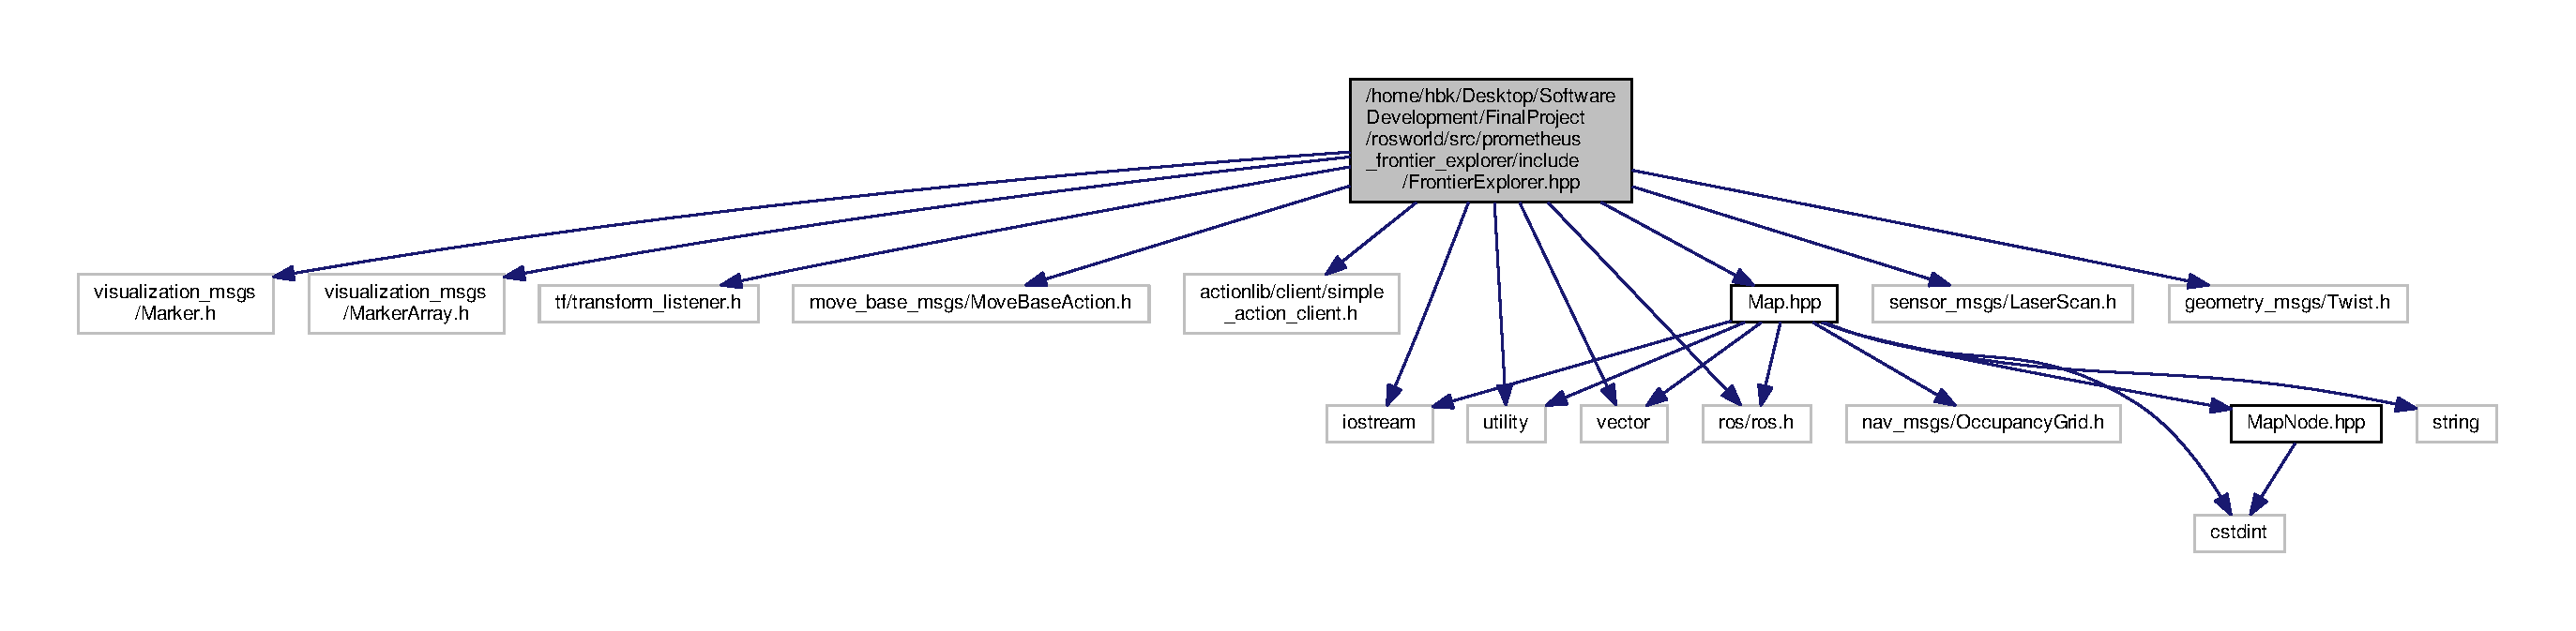
\includegraphics[width=350pt]{FrontierExplorer_8hpp__incl}
\end{center}
\end{figure}
This graph shows which files directly or indirectly include this file\+:
\nopagebreak
\begin{figure}[H]
\begin{center}
\leavevmode
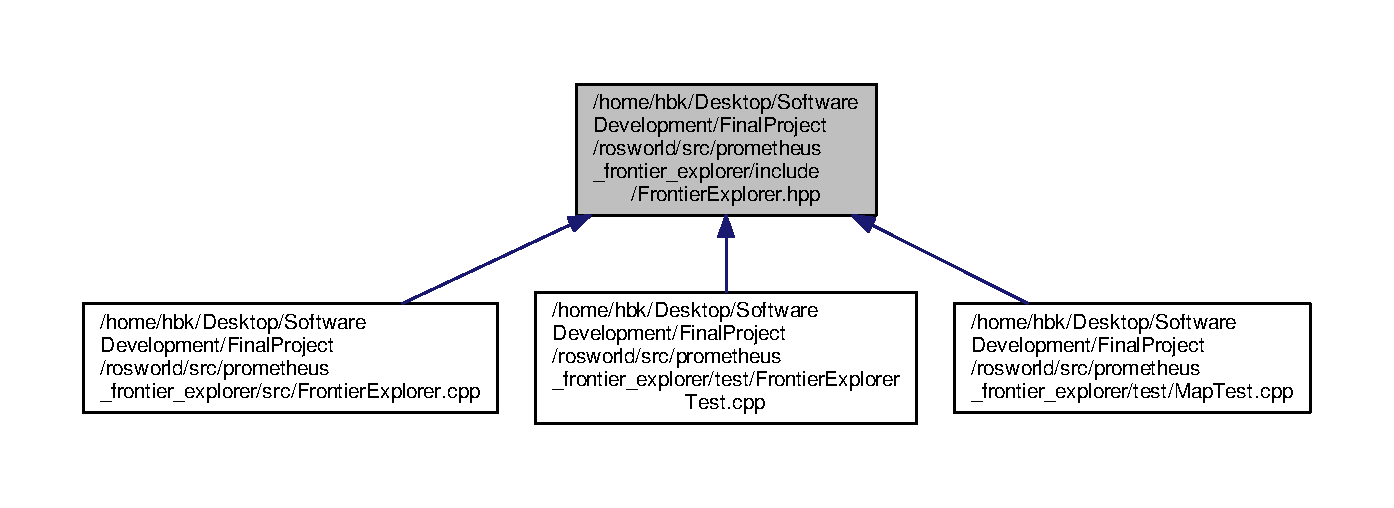
\includegraphics[width=350pt]{FrontierExplorer_8hpp__dep__incl}
\end{center}
\end{figure}
\subsection*{Classes}
\begin{DoxyCompactItemize}
\item 
class \hyperlink{classFrontierExplorer}{Frontier\+Explorer}
\begin{DoxyCompactList}\small\item\em Frontier\+Exploration Class. \end{DoxyCompactList}\end{DoxyCompactItemize}


\subsection{Detailed Description}
\hyperlink{classFrontierExplorer}{Frontier\+Explorer} header file. 

\begin{DoxyAuthor}{Author}
Harsh Kakashaniya and Rohitkrishna Nambiar 
\end{DoxyAuthor}
\begin{DoxyDate}{Date}
12/04/2018 
\end{DoxyDate}
\begin{DoxyVersion}{Version}
1.\+0 
\end{DoxyVersion}
\begin{DoxyCopyright}{Copyright}
B\+SD 3-\/\+Clause
\end{DoxyCopyright}
\hypertarget{MapTest_8cpp_DESCRIPTION}{}\subsection{D\+E\+S\+C\+R\+I\+P\+T\+I\+ON}\label{MapTest_8cpp_DESCRIPTION}
\hyperlink{classFrontierExplorer}{Frontier\+Explorer} class header declaration 
\hypertarget{Map_8hpp}{}\section{/home/hbk/\+Desktop/\+Software\+Development/\+Final\+Project/rosworld/src/prometheus\+\_\+frontier\+\_\+explorer/include/\+Map.hpp File Reference}
\label{Map_8hpp}\index{/home/hbk/\+Desktop/\+Software\+Development/\+Final\+Project/rosworld/src/prometheus\+\_\+frontier\+\_\+explorer/include/\+Map.\+hpp@{/home/hbk/\+Desktop/\+Software\+Development/\+Final\+Project/rosworld/src/prometheus\+\_\+frontier\+\_\+explorer/include/\+Map.\+hpp}}


\hyperlink{classMap}{Map} class header file.  


{\ttfamily \#include $<$nav\+\_\+msgs/\+Occupancy\+Grid.\+h$>$}\\*
{\ttfamily \#include $<$iostream$>$}\\*
{\ttfamily \#include $<$vector$>$}\\*
{\ttfamily \#include $<$cstdint$>$}\\*
{\ttfamily \#include $<$string$>$}\\*
{\ttfamily \#include $<$utility$>$}\\*
{\ttfamily \#include \char`\"{}ros/ros.\+h\char`\"{}}\\*
{\ttfamily \#include \char`\"{}Map\+Node.\+hpp\char`\"{}}\\*
Include dependency graph for Map.\+hpp\+:
\nopagebreak
\begin{figure}[H]
\begin{center}
\leavevmode
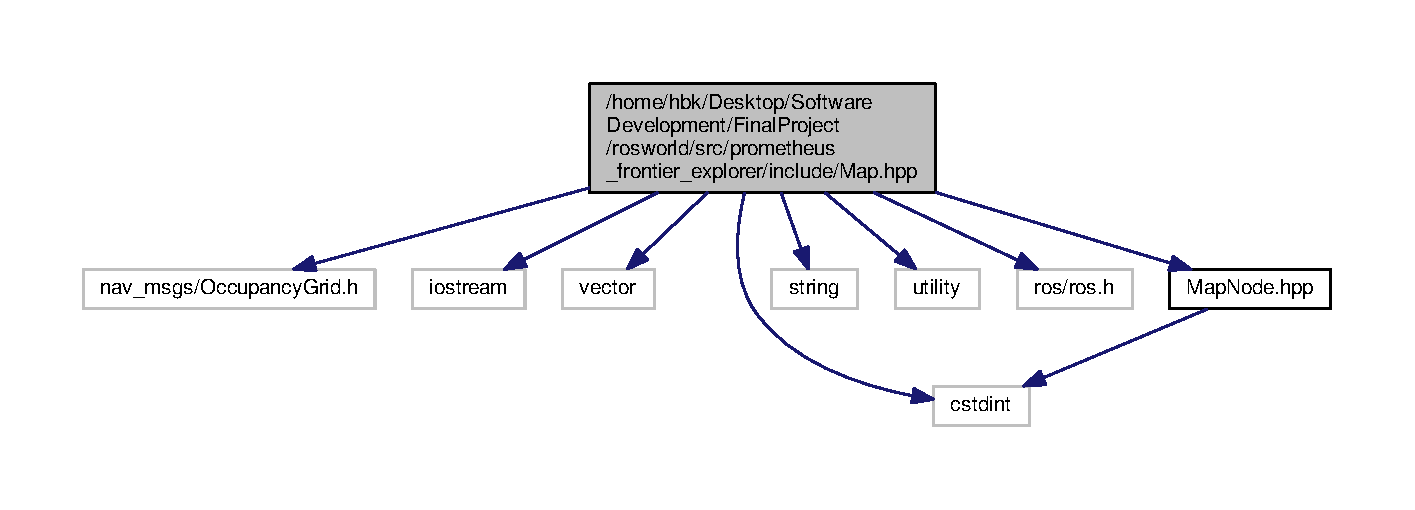
\includegraphics[width=350pt]{Map_8hpp__incl}
\end{center}
\end{figure}
This graph shows which files directly or indirectly include this file\+:
\nopagebreak
\begin{figure}[H]
\begin{center}
\leavevmode
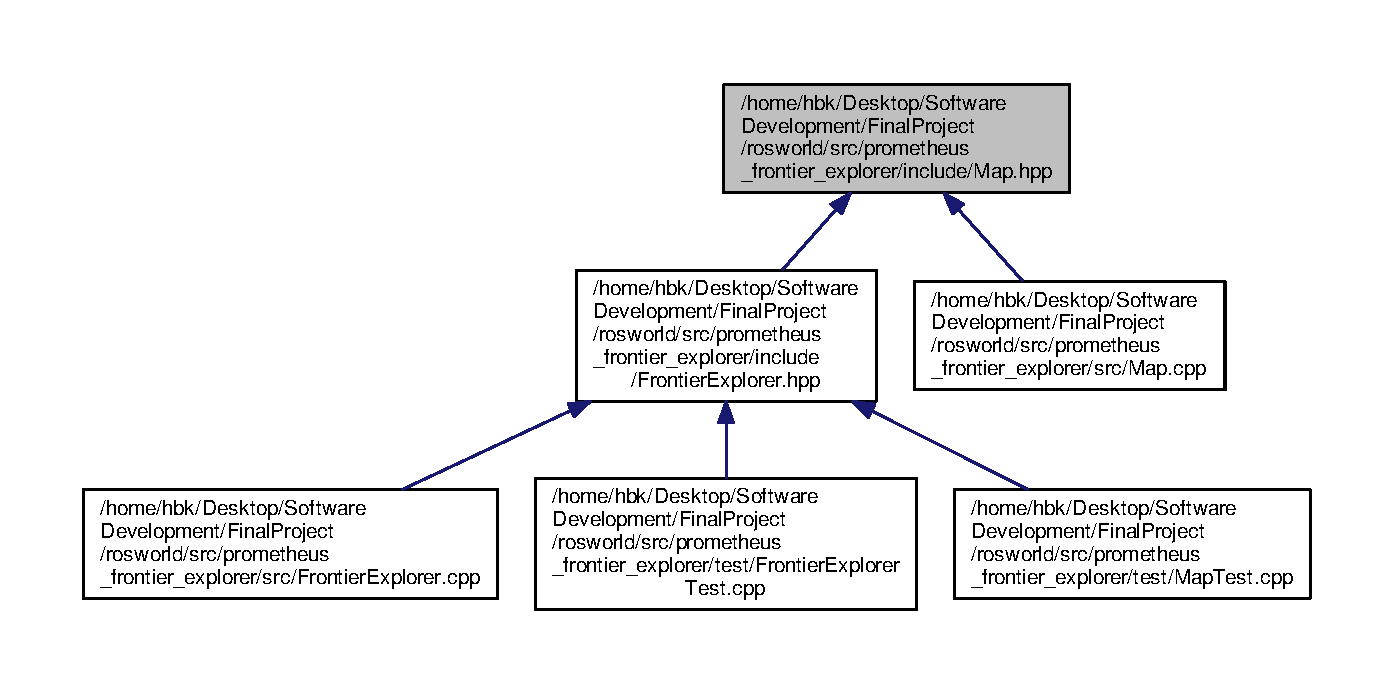
\includegraphics[width=350pt]{Map_8hpp__dep__incl}
\end{center}
\end{figure}
\subsection*{Classes}
\begin{DoxyCompactItemize}
\item 
class \hyperlink{classMap}{Map}
\begin{DoxyCompactList}\small\item\em \hyperlink{classMap}{Map} Class. \end{DoxyCompactList}\end{DoxyCompactItemize}


\subsection{Detailed Description}
\hyperlink{classMap}{Map} class header file. 

\begin{DoxyAuthor}{Author}
Harsh Kakashaniya and Rohitkrishna Nambiar 
\end{DoxyAuthor}
\begin{DoxyDate}{Date}
12/04/2018 
\end{DoxyDate}
\begin{DoxyVersion}{Version}
1.\+0 
\end{DoxyVersion}
\begin{DoxyCopyright}{Copyright}
B\+SD 3-\/\+Clause
\end{DoxyCopyright}
\hypertarget{MapTest_8cpp_DESCRIPTION}{}\subsection{D\+E\+S\+C\+R\+I\+P\+T\+I\+ON}\label{MapTest_8cpp_DESCRIPTION}
\hyperlink{classMap}{Map} class header declaration 
\hypertarget{MapNode_8hpp}{}\section{/home/hbk/\+Desktop/\+Software\+Development/\+Final\+Project/rosworld/src/prometheus\+\_\+frontier\+\_\+explorer/include/\+Map\+Node.hpp File Reference}
\label{MapNode_8hpp}\index{/home/hbk/\+Desktop/\+Software\+Development/\+Final\+Project/rosworld/src/prometheus\+\_\+frontier\+\_\+explorer/include/\+Map\+Node.\+hpp@{/home/hbk/\+Desktop/\+Software\+Development/\+Final\+Project/rosworld/src/prometheus\+\_\+frontier\+\_\+explorer/include/\+Map\+Node.\+hpp}}


\hyperlink{classMapNode}{Map\+Node} class header file.  


{\ttfamily \#include $<$cstdint$>$}\\*
Include dependency graph for Map\+Node.\+hpp\+:
\nopagebreak
\begin{figure}[H]
\begin{center}
\leavevmode
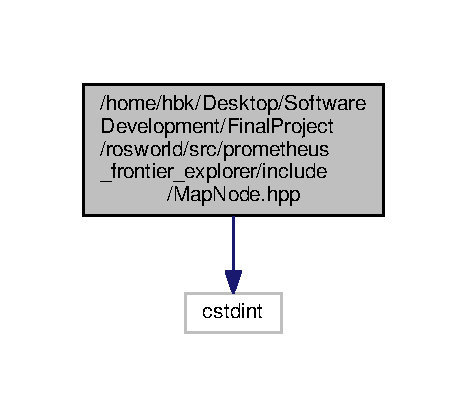
\includegraphics[width=224pt]{MapNode_8hpp__incl}
\end{center}
\end{figure}
This graph shows which files directly or indirectly include this file\+:
\nopagebreak
\begin{figure}[H]
\begin{center}
\leavevmode
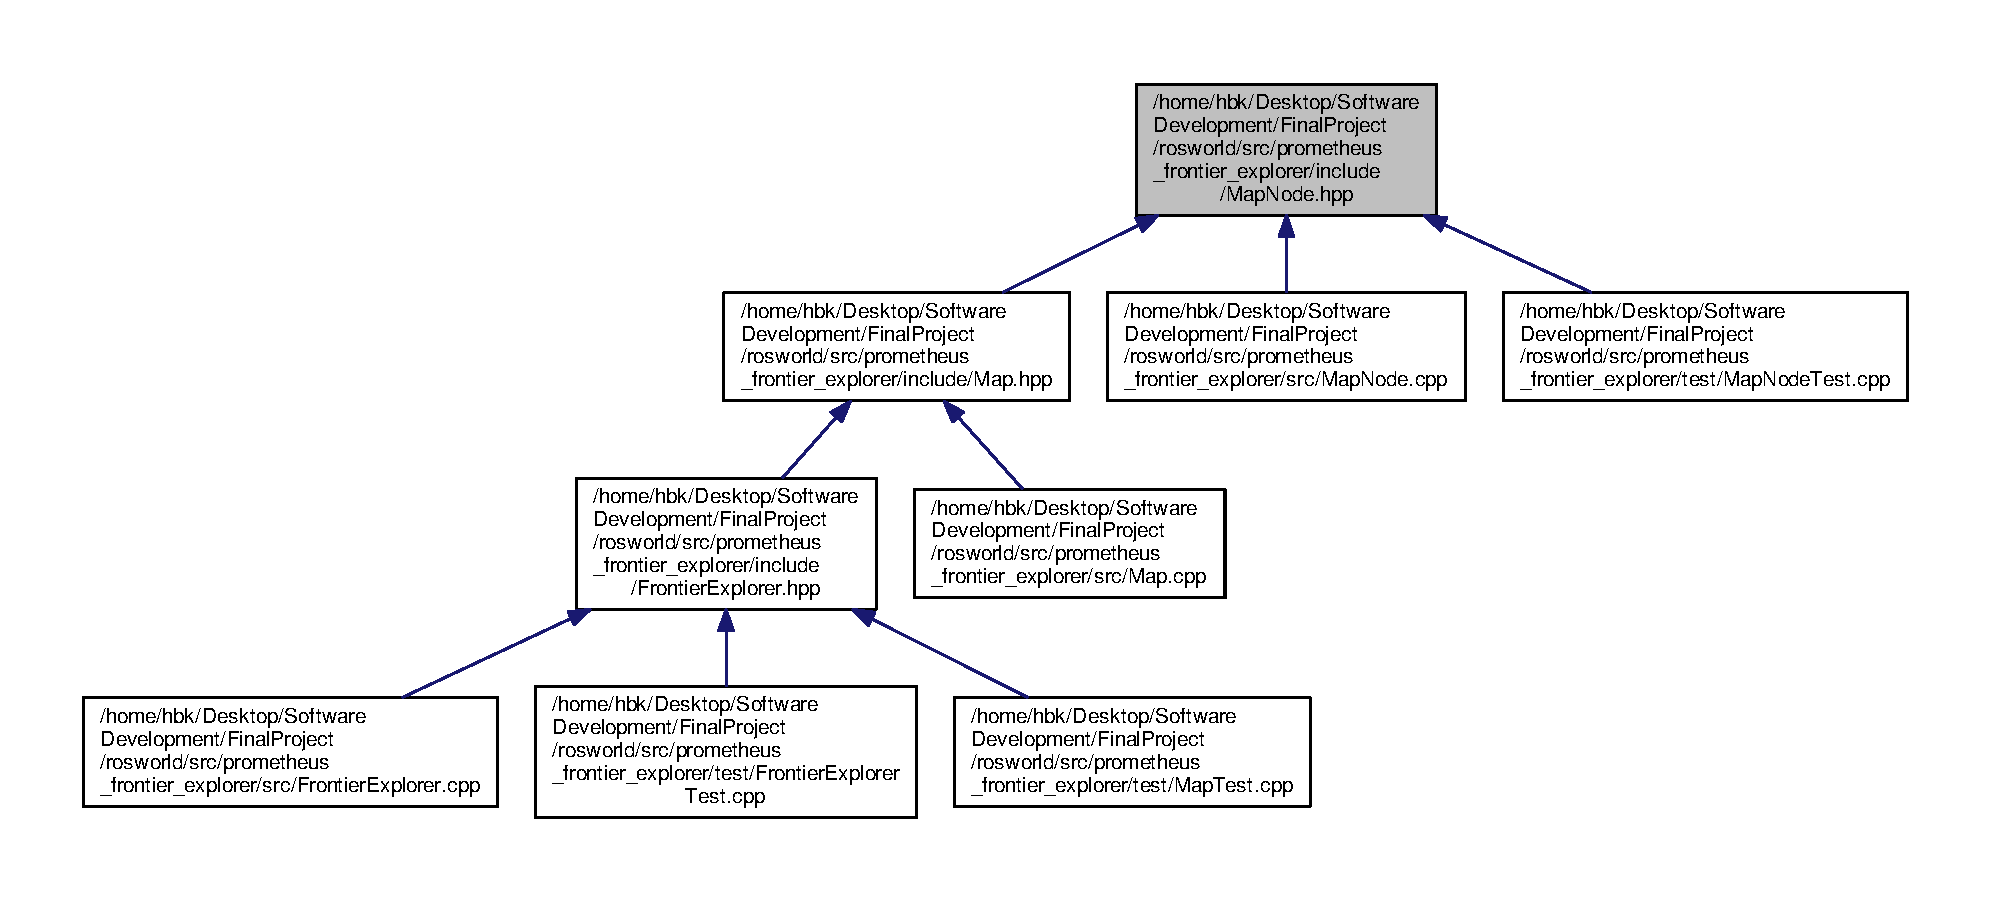
\includegraphics[width=350pt]{MapNode_8hpp__dep__incl}
\end{center}
\end{figure}
\subsection*{Classes}
\begin{DoxyCompactItemize}
\item 
class \hyperlink{classMapNode}{Map\+Node}
\begin{DoxyCompactList}\small\item\em \hyperlink{classMapNode}{Map\+Node} Class. \end{DoxyCompactList}\end{DoxyCompactItemize}


\subsection{Detailed Description}
\hyperlink{classMapNode}{Map\+Node} class header file. 

\begin{DoxyAuthor}{Author}
Harsh Kakashaniya and Rohitkrishna Nambiar 
\end{DoxyAuthor}
\begin{DoxyDate}{Date}
12/04/2018 
\end{DoxyDate}
\begin{DoxyVersion}{Version}
1.\+0 
\end{DoxyVersion}
\begin{DoxyCopyright}{Copyright}
B\+SD 3-\/\+Clause
\end{DoxyCopyright}
\hypertarget{MapTest_8cpp_DESCRIPTION}{}\subsection{D\+E\+S\+C\+R\+I\+P\+T\+I\+ON}\label{MapTest_8cpp_DESCRIPTION}
\hyperlink{classMapNode}{Map\+Node} class header declaration 
\hypertarget{FrontierExplorer_8cpp}{}\section{/home/hbk/\+Desktop/\+Software\+Development/\+Final\+Project/rosworld/src/prometheus\+\_\+frontier\+\_\+explorer/src/\+Frontier\+Explorer.cpp File Reference}
\label{FrontierExplorer_8cpp}\index{/home/hbk/\+Desktop/\+Software\+Development/\+Final\+Project/rosworld/src/prometheus\+\_\+frontier\+\_\+explorer/src/\+Frontier\+Explorer.\+cpp@{/home/hbk/\+Desktop/\+Software\+Development/\+Final\+Project/rosworld/src/prometheus\+\_\+frontier\+\_\+explorer/src/\+Frontier\+Explorer.\+cpp}}


\hyperlink{classFrontierExplorer}{Frontier\+Explorer} class.  


{\ttfamily \#include \char`\"{}Frontier\+Explorer.\+hpp\char`\"{}}\\*
{\ttfamily \#include $<$visualization\+\_\+msgs/\+Marker.\+h$>$}\\*
{\ttfamily \#include $<$visualization\+\_\+msgs/\+Marker\+Array.\+h$>$}\\*
{\ttfamily \#include $<$tf/transform\+\_\+listener.\+h$>$}\\*
{\ttfamily \#include $<$move\+\_\+base\+\_\+msgs/\+Move\+Base\+Action.\+h$>$}\\*
{\ttfamily \#include $<$actionlib/client/simple\+\_\+action\+\_\+client.\+h$>$}\\*
{\ttfamily \#include $<$iostream$>$}\\*
{\ttfamily \#include $<$utility$>$}\\*
{\ttfamily \#include $<$vector$>$}\\*
{\ttfamily \#include \char`\"{}ros/ros.\+h\char`\"{}}\\*
{\ttfamily \#include \char`\"{}sensor\+\_\+msgs/\+Laser\+Scan.\+h\char`\"{}}\\*
{\ttfamily \#include \char`\"{}geometry\+\_\+msgs/\+Twist.\+h\char`\"{}}\\*
Include dependency graph for Frontier\+Explorer.\+cpp\+:
\nopagebreak
\begin{figure}[H]
\begin{center}
\leavevmode
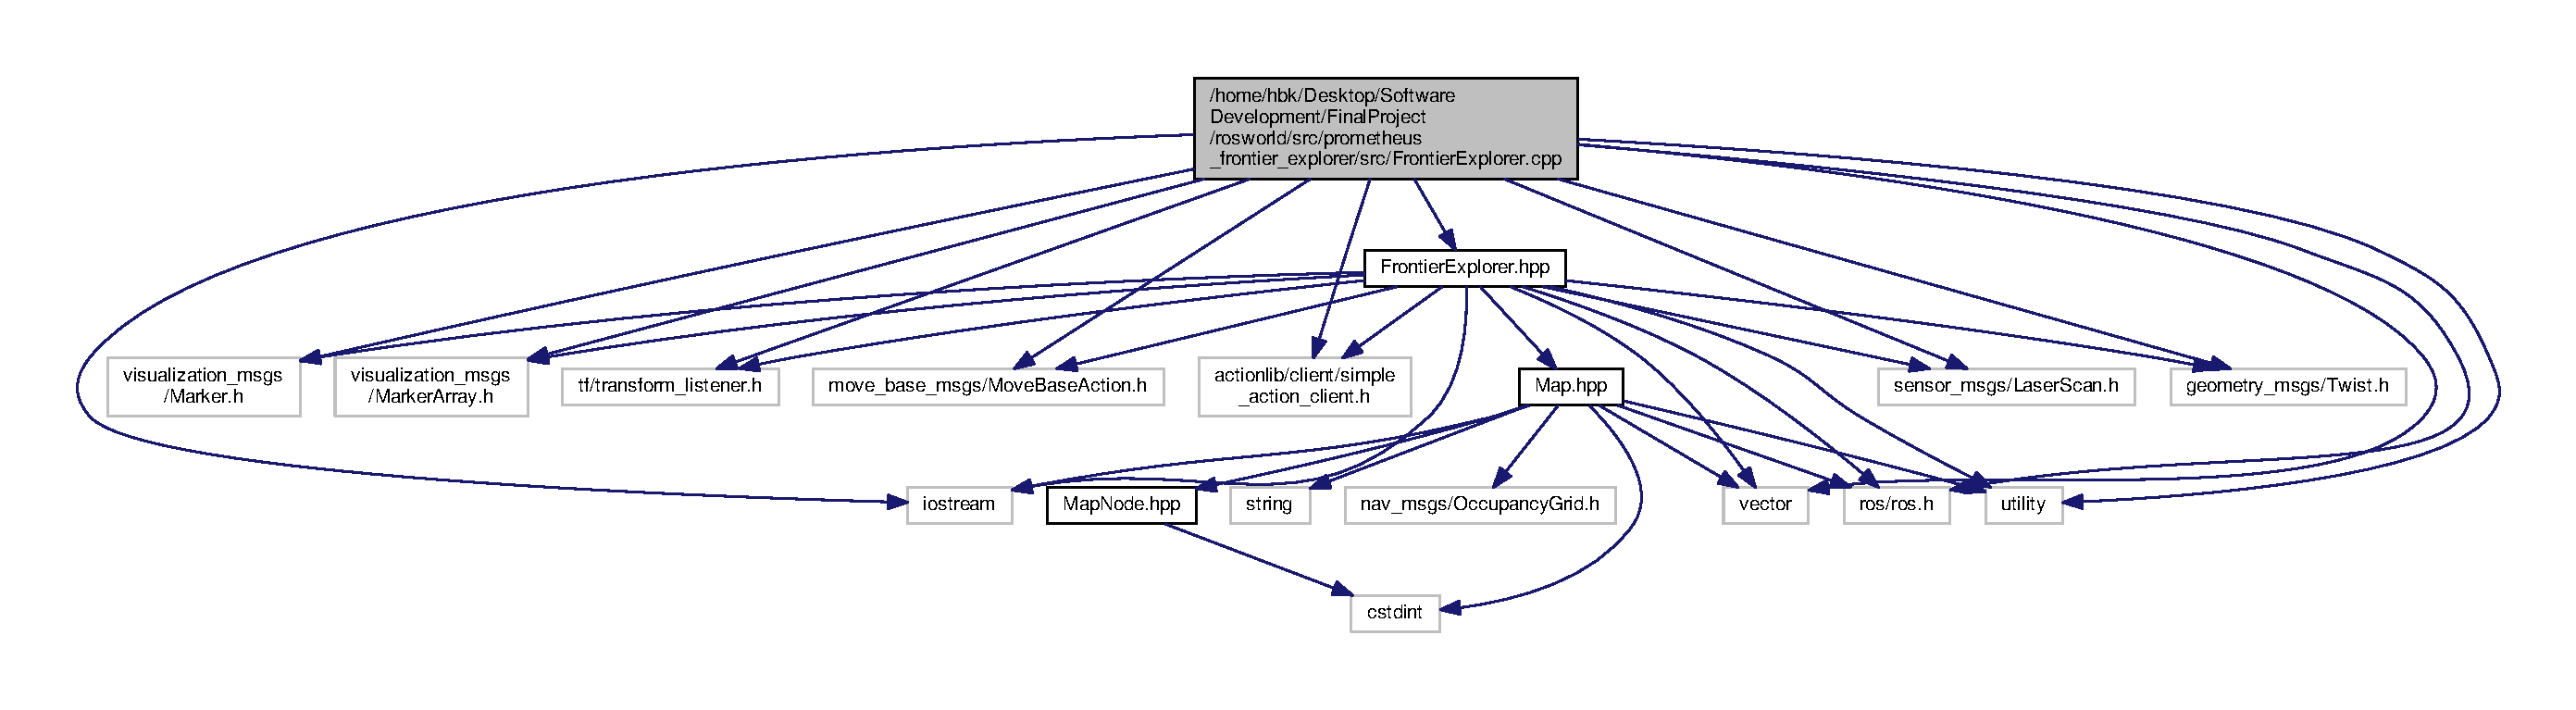
\includegraphics[width=350pt]{FrontierExplorer_8cpp__incl}
\end{center}
\end{figure}


\subsection{Detailed Description}
\hyperlink{classFrontierExplorer}{Frontier\+Explorer} class. 

\begin{DoxyAuthor}{Author}
Harsh Kakashaniya and Rohitkrishna Nambiar 
\end{DoxyAuthor}
\begin{DoxyDate}{Date}
12/04/2018 
\end{DoxyDate}
\begin{DoxyVersion}{Version}
1.\+0 
\end{DoxyVersion}
\begin{DoxyCopyright}{Copyright}
B\+SD 3-\/\+Clause
\end{DoxyCopyright}
\hypertarget{MapTest_8cpp_DESCRIPTION}{}\subsection{D\+E\+S\+C\+R\+I\+P\+T\+I\+ON}\label{MapTest_8cpp_DESCRIPTION}
\hyperlink{classFrontierExplorer}{Frontier\+Explorer} class implementation 
\hypertarget{Map_8cpp}{}\section{/home/hbk/\+Desktop/\+Software\+Development/\+Final\+Project/rosworld/src/prometheus\+\_\+frontier\+\_\+explorer/src/\+Map.cpp File Reference}
\label{Map_8cpp}\index{/home/hbk/\+Desktop/\+Software\+Development/\+Final\+Project/rosworld/src/prometheus\+\_\+frontier\+\_\+explorer/src/\+Map.\+cpp@{/home/hbk/\+Desktop/\+Software\+Development/\+Final\+Project/rosworld/src/prometheus\+\_\+frontier\+\_\+explorer/src/\+Map.\+cpp}}


\hyperlink{classMap}{Map} class implementation file.  


{\ttfamily \#include \char`\"{}Map.\+hpp\char`\"{}}\\*
{\ttfamily \#include $<$nav\+\_\+msgs/\+Occupancy\+Grid.\+h$>$}\\*
{\ttfamily \#include $<$iostream$>$}\\*
{\ttfamily \#include $<$vector$>$}\\*
{\ttfamily \#include $<$cstdint$>$}\\*
{\ttfamily \#include $<$string$>$}\\*
{\ttfamily \#include $<$utility$>$}\\*
Include dependency graph for Map.\+cpp\+:
\nopagebreak
\begin{figure}[H]
\begin{center}
\leavevmode
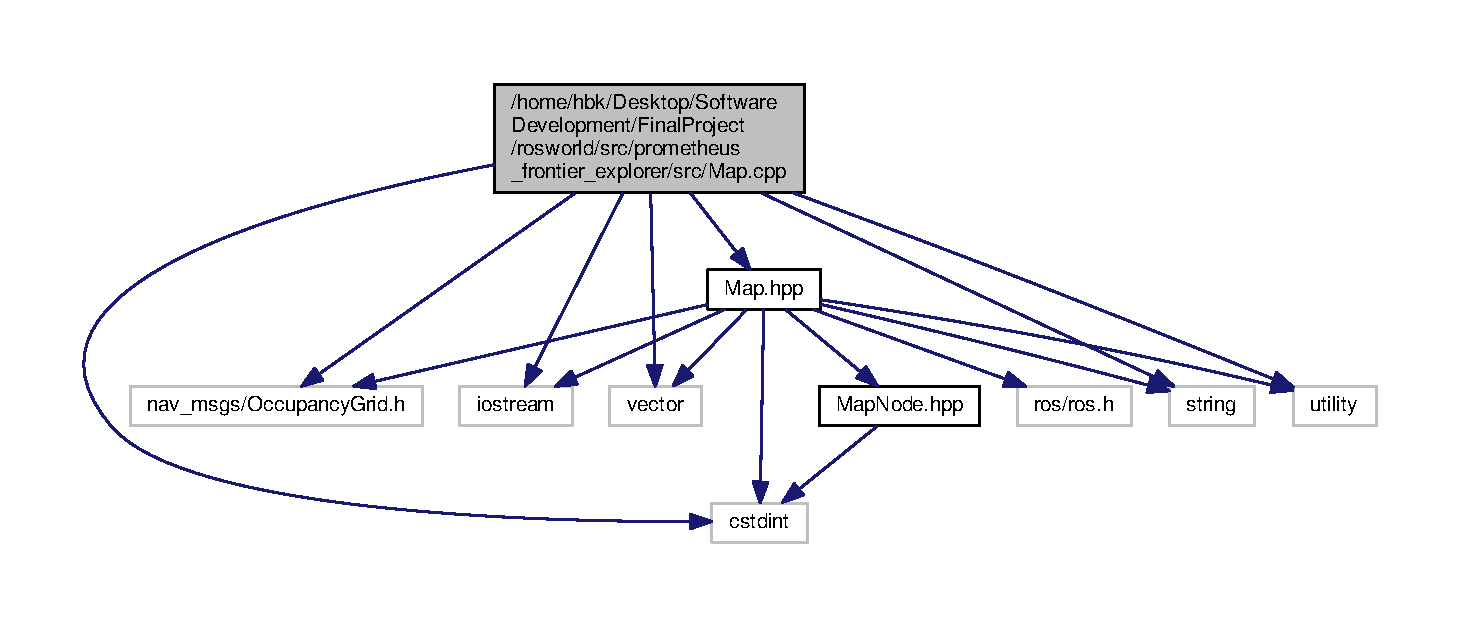
\includegraphics[width=350pt]{Map_8cpp__incl}
\end{center}
\end{figure}


\subsection{Detailed Description}
\hyperlink{classMap}{Map} class implementation file. 

\begin{DoxyAuthor}{Author}
Harsh Kakashaniya and Rohitkrishna Nambiar 
\end{DoxyAuthor}
\begin{DoxyDate}{Date}
12/04/2018 
\end{DoxyDate}
\begin{DoxyVersion}{Version}
1.\+0 
\end{DoxyVersion}
\begin{DoxyCopyright}{Copyright}
B\+SD 3-\/\+Clause
\end{DoxyCopyright}
\hypertarget{MapTest_8cpp_DESCRIPTION}{}\subsection{D\+E\+S\+C\+R\+I\+P\+T\+I\+ON}\label{MapTest_8cpp_DESCRIPTION}
\hyperlink{classMap}{Map} class implementation 
\hypertarget{MapNode_8cpp}{}\section{/home/hbk/\+Desktop/\+Software\+Development/\+Final\+Project/rosworld/src/prometheus\+\_\+frontier\+\_\+explorer/src/\+Map\+Node.cpp File Reference}
\label{MapNode_8cpp}\index{/home/hbk/\+Desktop/\+Software\+Development/\+Final\+Project/rosworld/src/prometheus\+\_\+frontier\+\_\+explorer/src/\+Map\+Node.\+cpp@{/home/hbk/\+Desktop/\+Software\+Development/\+Final\+Project/rosworld/src/prometheus\+\_\+frontier\+\_\+explorer/src/\+Map\+Node.\+cpp}}


\hyperlink{classMapNode}{Map\+Node} class implementation file.  


{\ttfamily \#include \char`\"{}Map\+Node.\+hpp\char`\"{}}\\*
{\ttfamily \#include $<$cstdint$>$}\\*
Include dependency graph for Map\+Node.\+cpp\+:
\nopagebreak
\begin{figure}[H]
\begin{center}
\leavevmode
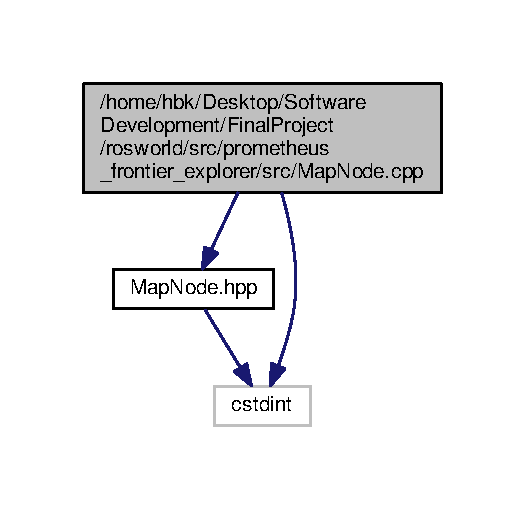
\includegraphics[width=252pt]{MapNode_8cpp__incl}
\end{center}
\end{figure}


\subsection{Detailed Description}
\hyperlink{classMapNode}{Map\+Node} class implementation file. 

\begin{DoxyAuthor}{Author}
Harsh Kakashaniya and Rohitkrishna Nambiar 
\end{DoxyAuthor}
\begin{DoxyDate}{Date}
12/04/2018 
\end{DoxyDate}
\begin{DoxyVersion}{Version}
1.\+0 
\end{DoxyVersion}
\begin{DoxyCopyright}{Copyright}
B\+SD 3-\/\+Clause
\end{DoxyCopyright}
\hypertarget{MapTest_8cpp_DESCRIPTION}{}\subsection{D\+E\+S\+C\+R\+I\+P\+T\+I\+ON}\label{MapTest_8cpp_DESCRIPTION}
Mapnode class implementation file for prometheus\+\_\+frontier\+\_\+exploration package. 
\hypertarget{FrontierExplorerTest_8cpp}{}\section{/home/hbk/\+Desktop/\+Software\+Development/\+Final\+Project/rosworld/src/prometheus\+\_\+frontier\+\_\+explorer/test/\+Frontier\+Explorer\+Test.cpp File Reference}
\label{FrontierExplorerTest_8cpp}\index{/home/hbk/\+Desktop/\+Software\+Development/\+Final\+Project/rosworld/src/prometheus\+\_\+frontier\+\_\+explorer/test/\+Frontier\+Explorer\+Test.\+cpp@{/home/hbk/\+Desktop/\+Software\+Development/\+Final\+Project/rosworld/src/prometheus\+\_\+frontier\+\_\+explorer/test/\+Frontier\+Explorer\+Test.\+cpp}}


Test for \hyperlink{classFrontierExplorer}{Frontier\+Explorer} class file.  


{\ttfamily \#include $<$gtest/gtest.\+h$>$}\\*
{\ttfamily \#include \char`\"{}Frontier\+Explorer.\+hpp\char`\"{}}\\*
{\ttfamily \#include \char`\"{}ros/ros.\+h\char`\"{}}\\*
Include dependency graph for Frontier\+Explorer\+Test.\+cpp\+:
\nopagebreak
\begin{figure}[H]
\begin{center}
\leavevmode
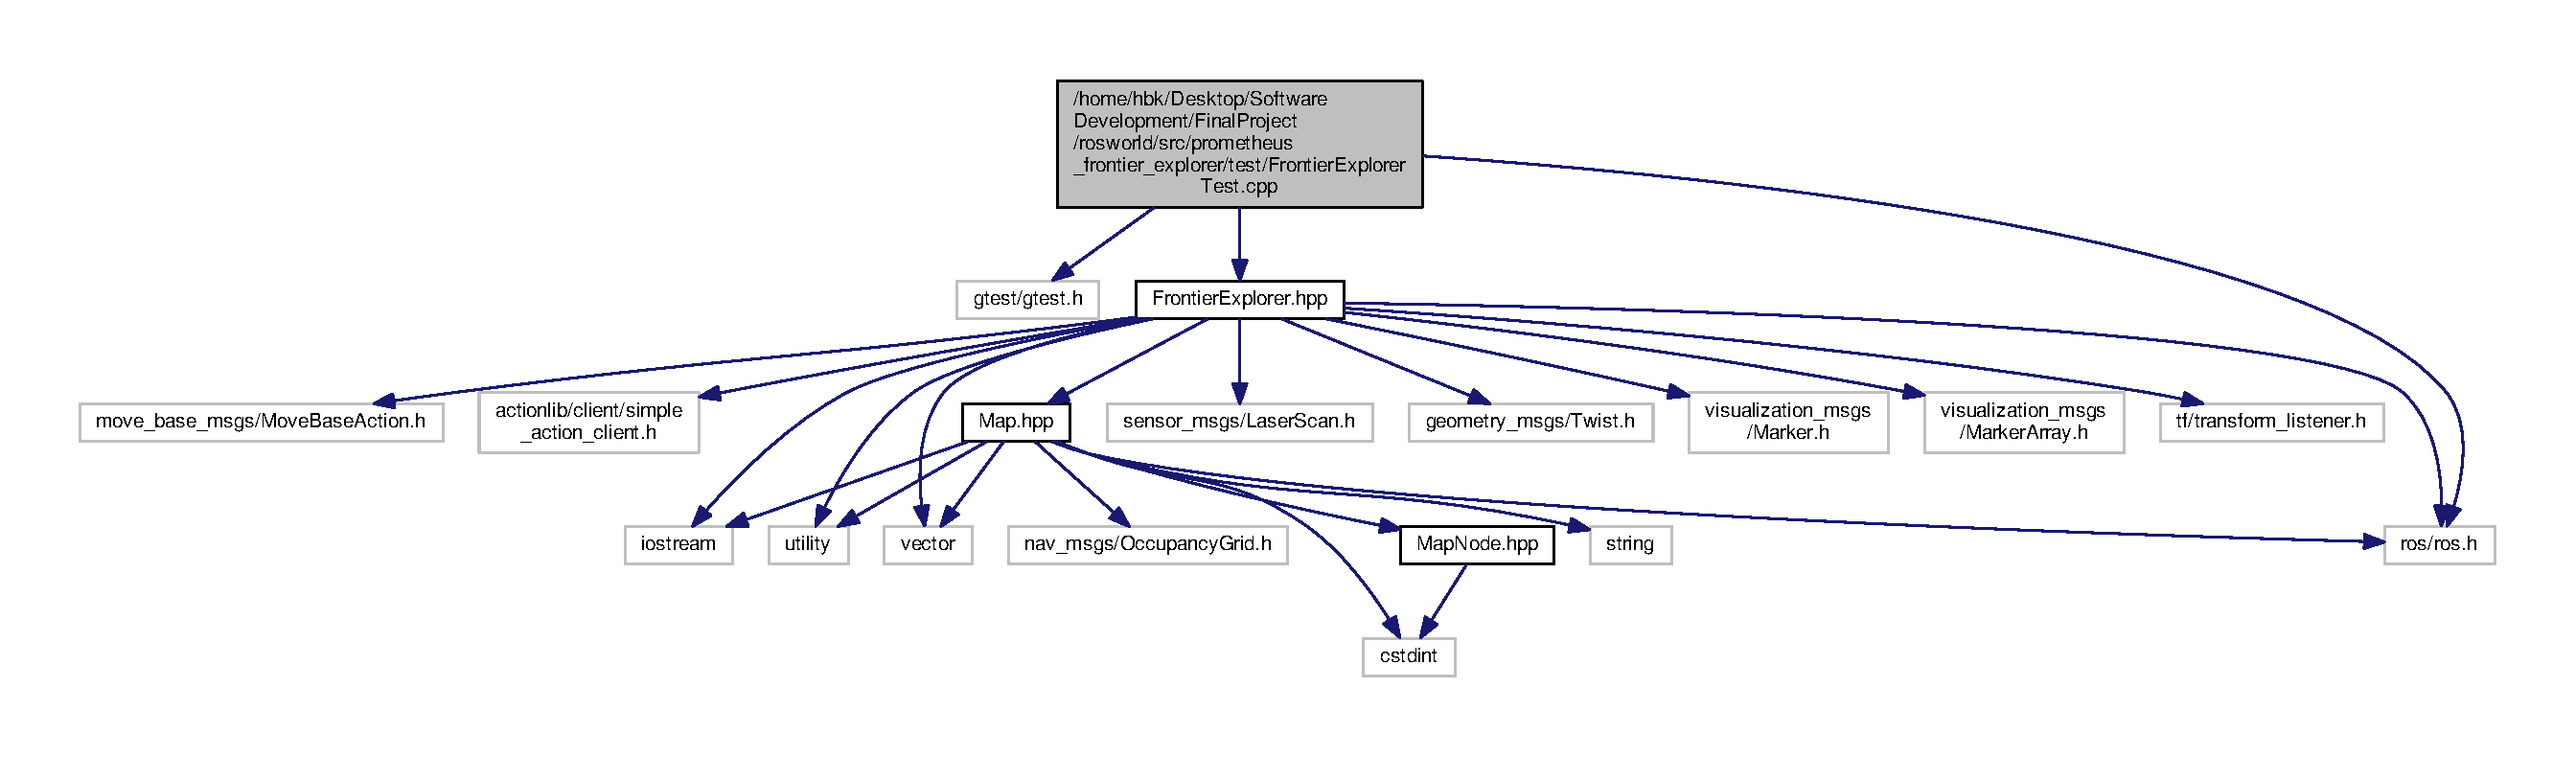
\includegraphics[width=350pt]{FrontierExplorerTest_8cpp__incl}
\end{center}
\end{figure}
\subsection*{Classes}
\begin{DoxyCompactItemize}
\item 
class \hyperlink{classTestSubPub}{Test\+Sub\+Pub}
\begin{DoxyCompactList}\small\item\em \hyperlink{classTestSubPub}{Test\+Sub\+Pub} Class. \end{DoxyCompactList}\item 
class \hyperlink{classFrontierExplorerTest}{Frontier\+Explorer\+Test}
\begin{DoxyCompactList}\small\item\em \hyperlink{classFrontierExplorerTest}{Frontier\+Explorer\+Test} Class. \end{DoxyCompactList}\end{DoxyCompactItemize}
\subsection*{Functions}
\begin{DoxyCompactItemize}
\item 
\hyperlink{FrontierExplorerTest_8cpp_ade8e9bd8c68b859ef8ced199102f1e7b}{T\+E\+S\+T\+\_\+F} (\hyperlink{classFrontierExplorerTest}{Frontier\+Explorer\+Test}, test\+All\+Marker\+Publish)
\begin{DoxyCompactList}\small\item\em Test all frontier marker publisher. \end{DoxyCompactList}\item 
\hyperlink{FrontierExplorerTest_8cpp_ab7299c0f700020052d8be3ce8da72cf2}{T\+E\+S\+T\+\_\+F} (\hyperlink{classFrontierExplorerTest}{Frontier\+Explorer\+Test}, test\+Frontier\+Segmented\+Publish)
\begin{DoxyCompactList}\small\item\em Test segmented frontier marker publisher. \end{DoxyCompactList}\item 
\hyperlink{FrontierExplorerTest_8cpp_a9d3e9d55aa0d185a8f0f3ce54ff9141c}{T\+E\+S\+T\+\_\+F} (\hyperlink{classFrontierExplorerTest}{Frontier\+Explorer\+Test}, test\+Frontier\+Clustered\+Publish)
\begin{DoxyCompactList}\small\item\em Test frontier clusters marker publisher. \end{DoxyCompactList}\item 
\hyperlink{FrontierExplorerTest_8cpp_af2156fb9cbdee4df4de618f9209bb259}{T\+E\+S\+T\+\_\+F} (\hyperlink{classFrontierExplorerTest}{Frontier\+Explorer\+Test}, test\+Reach\+Avoid\+Publish)
\begin{DoxyCompactList}\small\item\em Test reach avoid marker publisher. \end{DoxyCompactList}\item 
\hyperlink{FrontierExplorerTest_8cpp_a0415ed9323b0f85bfff8dbc59dc73155}{T\+E\+S\+T\+\_\+F} (\hyperlink{classFrontierExplorerTest}{Frontier\+Explorer\+Test}, test\+Vel\+Publish)
\begin{DoxyCompactList}\small\item\em Test turtlebot velocity publisher. \end{DoxyCompactList}\item 
\hyperlink{FrontierExplorerTest_8cpp_a9e5e93d641834a0d480748ac33309b63}{T\+E\+S\+T\+\_\+F} (\hyperlink{classFrontierExplorerTest}{Frontier\+Explorer\+Test}, test\+Grid\+Subscriber)
\begin{DoxyCompactList}\small\item\em Test occupancy grid map subscriber. \end{DoxyCompactList}\end{DoxyCompactItemize}


\subsection{Detailed Description}
Test for \hyperlink{classFrontierExplorer}{Frontier\+Explorer} class file. 

\begin{DoxyAuthor}{Author}
Harsh Kakashaniya and Rohitkrishna Nambiar 
\end{DoxyAuthor}
\begin{DoxyDate}{Date}
12/04/2018 
\end{DoxyDate}
\begin{DoxyVersion}{Version}
1.\+0 
\end{DoxyVersion}
\begin{DoxyCopyright}{Copyright}
B\+SD 3-\/\+Clause
\end{DoxyCopyright}
\hypertarget{MapTest_8cpp_DESCRIPTION}{}\subsection{D\+E\+S\+C\+R\+I\+P\+T\+I\+ON}\label{MapTest_8cpp_DESCRIPTION}
Test implementation for \hyperlink{classFrontierExplorer}{Frontier\+Explorer} class 

\subsection{Function Documentation}
\index{Frontier\+Explorer\+Test.\+cpp@{Frontier\+Explorer\+Test.\+cpp}!T\+E\+S\+T\+\_\+F@{T\+E\+S\+T\+\_\+F}}
\index{T\+E\+S\+T\+\_\+F@{T\+E\+S\+T\+\_\+F}!Frontier\+Explorer\+Test.\+cpp@{Frontier\+Explorer\+Test.\+cpp}}
\subsubsection[{\texorpdfstring{T\+E\+S\+T\+\_\+\+F(\+Frontier\+Explorer\+Test, test\+All\+Marker\+Publish)}{TEST_F(FrontierExplorerTest, testAllMarkerPublish)}}]{\setlength{\rightskip}{0pt plus 5cm}T\+E\+S\+T\+\_\+F (
\begin{DoxyParamCaption}
\item[{{\bf Frontier\+Explorer\+Test}}]{, }
\item[{test\+All\+Marker\+Publish}]{}
\end{DoxyParamCaption}
)}\hypertarget{FrontierExplorerTest_8cpp_ade8e9bd8c68b859ef8ced199102f1e7b}{}\label{FrontierExplorerTest_8cpp_ade8e9bd8c68b859ef8ced199102f1e7b}


Test all frontier marker publisher. 


\begin{DoxyParams}{Parameters}
{\em none} & \\
\hline
\end{DoxyParams}
\begin{DoxyReturn}{Returns}
none 
\end{DoxyReturn}
\index{Frontier\+Explorer\+Test.\+cpp@{Frontier\+Explorer\+Test.\+cpp}!T\+E\+S\+T\+\_\+F@{T\+E\+S\+T\+\_\+F}}
\index{T\+E\+S\+T\+\_\+F@{T\+E\+S\+T\+\_\+F}!Frontier\+Explorer\+Test.\+cpp@{Frontier\+Explorer\+Test.\+cpp}}
\subsubsection[{\texorpdfstring{T\+E\+S\+T\+\_\+\+F(\+Frontier\+Explorer\+Test, test\+Frontier\+Segmented\+Publish)}{TEST_F(FrontierExplorerTest, testFrontierSegmentedPublish)}}]{\setlength{\rightskip}{0pt plus 5cm}T\+E\+S\+T\+\_\+F (
\begin{DoxyParamCaption}
\item[{{\bf Frontier\+Explorer\+Test}}]{, }
\item[{test\+Frontier\+Segmented\+Publish}]{}
\end{DoxyParamCaption}
)}\hypertarget{FrontierExplorerTest_8cpp_ab7299c0f700020052d8be3ce8da72cf2}{}\label{FrontierExplorerTest_8cpp_ab7299c0f700020052d8be3ce8da72cf2}


Test segmented frontier marker publisher. 


\begin{DoxyParams}{Parameters}
{\em none} & \\
\hline
\end{DoxyParams}
\begin{DoxyReturn}{Returns}
none 
\end{DoxyReturn}
\index{Frontier\+Explorer\+Test.\+cpp@{Frontier\+Explorer\+Test.\+cpp}!T\+E\+S\+T\+\_\+F@{T\+E\+S\+T\+\_\+F}}
\index{T\+E\+S\+T\+\_\+F@{T\+E\+S\+T\+\_\+F}!Frontier\+Explorer\+Test.\+cpp@{Frontier\+Explorer\+Test.\+cpp}}
\subsubsection[{\texorpdfstring{T\+E\+S\+T\+\_\+\+F(\+Frontier\+Explorer\+Test, test\+Frontier\+Clustered\+Publish)}{TEST_F(FrontierExplorerTest, testFrontierClusteredPublish)}}]{\setlength{\rightskip}{0pt plus 5cm}T\+E\+S\+T\+\_\+F (
\begin{DoxyParamCaption}
\item[{{\bf Frontier\+Explorer\+Test}}]{, }
\item[{test\+Frontier\+Clustered\+Publish}]{}
\end{DoxyParamCaption}
)}\hypertarget{FrontierExplorerTest_8cpp_a9d3e9d55aa0d185a8f0f3ce54ff9141c}{}\label{FrontierExplorerTest_8cpp_a9d3e9d55aa0d185a8f0f3ce54ff9141c}


Test frontier clusters marker publisher. 


\begin{DoxyParams}{Parameters}
{\em none} & \\
\hline
\end{DoxyParams}
\begin{DoxyReturn}{Returns}
none 
\end{DoxyReturn}
\index{Frontier\+Explorer\+Test.\+cpp@{Frontier\+Explorer\+Test.\+cpp}!T\+E\+S\+T\+\_\+F@{T\+E\+S\+T\+\_\+F}}
\index{T\+E\+S\+T\+\_\+F@{T\+E\+S\+T\+\_\+F}!Frontier\+Explorer\+Test.\+cpp@{Frontier\+Explorer\+Test.\+cpp}}
\subsubsection[{\texorpdfstring{T\+E\+S\+T\+\_\+\+F(\+Frontier\+Explorer\+Test, test\+Reach\+Avoid\+Publish)}{TEST_F(FrontierExplorerTest, testReachAvoidPublish)}}]{\setlength{\rightskip}{0pt plus 5cm}T\+E\+S\+T\+\_\+F (
\begin{DoxyParamCaption}
\item[{{\bf Frontier\+Explorer\+Test}}]{, }
\item[{test\+Reach\+Avoid\+Publish}]{}
\end{DoxyParamCaption}
)}\hypertarget{FrontierExplorerTest_8cpp_af2156fb9cbdee4df4de618f9209bb259}{}\label{FrontierExplorerTest_8cpp_af2156fb9cbdee4df4de618f9209bb259}


Test reach avoid marker publisher. 


\begin{DoxyParams}{Parameters}
{\em none} & \\
\hline
\end{DoxyParams}
\begin{DoxyReturn}{Returns}
none 
\end{DoxyReturn}
\index{Frontier\+Explorer\+Test.\+cpp@{Frontier\+Explorer\+Test.\+cpp}!T\+E\+S\+T\+\_\+F@{T\+E\+S\+T\+\_\+F}}
\index{T\+E\+S\+T\+\_\+F@{T\+E\+S\+T\+\_\+F}!Frontier\+Explorer\+Test.\+cpp@{Frontier\+Explorer\+Test.\+cpp}}
\subsubsection[{\texorpdfstring{T\+E\+S\+T\+\_\+\+F(\+Frontier\+Explorer\+Test, test\+Vel\+Publish)}{TEST_F(FrontierExplorerTest, testVelPublish)}}]{\setlength{\rightskip}{0pt plus 5cm}T\+E\+S\+T\+\_\+F (
\begin{DoxyParamCaption}
\item[{{\bf Frontier\+Explorer\+Test}}]{, }
\item[{test\+Vel\+Publish}]{}
\end{DoxyParamCaption}
)}\hypertarget{FrontierExplorerTest_8cpp_a0415ed9323b0f85bfff8dbc59dc73155}{}\label{FrontierExplorerTest_8cpp_a0415ed9323b0f85bfff8dbc59dc73155}


Test turtlebot velocity publisher. 


\begin{DoxyParams}{Parameters}
{\em none} & \\
\hline
\end{DoxyParams}
\begin{DoxyReturn}{Returns}
none 
\end{DoxyReturn}
\index{Frontier\+Explorer\+Test.\+cpp@{Frontier\+Explorer\+Test.\+cpp}!T\+E\+S\+T\+\_\+F@{T\+E\+S\+T\+\_\+F}}
\index{T\+E\+S\+T\+\_\+F@{T\+E\+S\+T\+\_\+F}!Frontier\+Explorer\+Test.\+cpp@{Frontier\+Explorer\+Test.\+cpp}}
\subsubsection[{\texorpdfstring{T\+E\+S\+T\+\_\+\+F(\+Frontier\+Explorer\+Test, test\+Grid\+Subscriber)}{TEST_F(FrontierExplorerTest, testGridSubscriber)}}]{\setlength{\rightskip}{0pt plus 5cm}T\+E\+S\+T\+\_\+F (
\begin{DoxyParamCaption}
\item[{{\bf Frontier\+Explorer\+Test}}]{, }
\item[{test\+Grid\+Subscriber}]{}
\end{DoxyParamCaption}
)}\hypertarget{FrontierExplorerTest_8cpp_a9e5e93d641834a0d480748ac33309b63}{}\label{FrontierExplorerTest_8cpp_a9e5e93d641834a0d480748ac33309b63}


Test occupancy grid map subscriber. 


\begin{DoxyParams}{Parameters}
{\em none} & \\
\hline
\end{DoxyParams}
\begin{DoxyReturn}{Returns}
none 
\end{DoxyReturn}

\hypertarget{MapNodeTest_8cpp}{}\section{/home/hbk/\+Desktop/\+Software\+Development/\+Final\+Project/rosworld/src/prometheus\+\_\+frontier\+\_\+explorer/test/\+Map\+Node\+Test.cpp File Reference}
\label{MapNodeTest_8cpp}\index{/home/hbk/\+Desktop/\+Software\+Development/\+Final\+Project/rosworld/src/prometheus\+\_\+frontier\+\_\+explorer/test/\+Map\+Node\+Test.\+cpp@{/home/hbk/\+Desktop/\+Software\+Development/\+Final\+Project/rosworld/src/prometheus\+\_\+frontier\+\_\+explorer/test/\+Map\+Node\+Test.\+cpp}}


Test for \hyperlink{classMapNode}{Map\+Node} class file.  


{\ttfamily \#include $<$gtest/gtest.\+h$>$}\\*
{\ttfamily \#include \char`\"{}Map\+Node.\+hpp\char`\"{}}\\*
Include dependency graph for Map\+Node\+Test.\+cpp\+:
\nopagebreak
\begin{figure}[H]
\begin{center}
\leavevmode
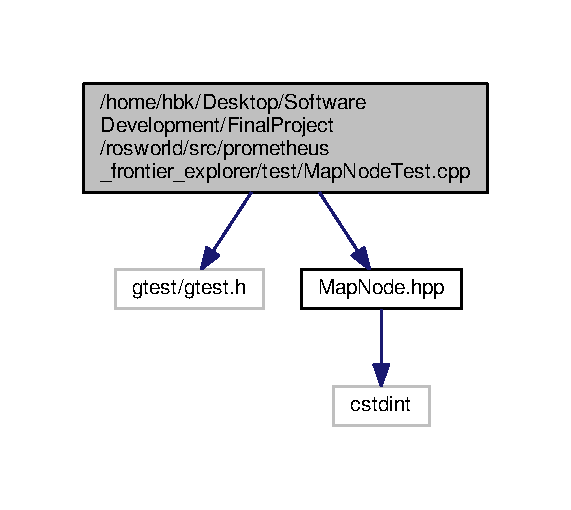
\includegraphics[width=274pt]{MapNodeTest_8cpp__incl}
\end{center}
\end{figure}
\subsection*{Classes}
\begin{DoxyCompactItemize}
\item 
class \hyperlink{classMapNodeTest}{Map\+Node\+Test}
\begin{DoxyCompactList}\small\item\em \hyperlink{classMapNodeTest}{Map\+Node\+Test} Class. \end{DoxyCompactList}\end{DoxyCompactItemize}
\subsection*{Functions}
\begin{DoxyCompactItemize}
\item 
\hyperlink{MapNodeTest_8cpp_a83409adb7098f343874d322df7162b62}{T\+E\+S\+T\+\_\+F} (\hyperlink{classMapNodeTest}{Map\+Node\+Test}, test\+SetX)
\begin{DoxyCompactList}\small\item\em Test set node x method. \end{DoxyCompactList}\item 
\hyperlink{MapNodeTest_8cpp_afc98396e4eefc3f8db1cdc22dc72bbeb}{T\+E\+S\+T\+\_\+F} (\hyperlink{classMapNodeTest}{Map\+Node\+Test}, test\+SetY)
\begin{DoxyCompactList}\small\item\em Test set node y method. \end{DoxyCompactList}\item 
\hyperlink{MapNodeTest_8cpp_a9616fa7265c0acf8db7deb67006bf4b3}{T\+E\+S\+T\+\_\+F} (\hyperlink{classMapNodeTest}{Map\+Node\+Test}, test\+Set\+Probability)
\begin{DoxyCompactList}\small\item\em Test set node probability method. \end{DoxyCompactList}\item 
\hyperlink{MapNodeTest_8cpp_a4363164aae44f4d8990a6f3d768c15f9}{T\+E\+S\+T\+\_\+F} (\hyperlink{classMapNodeTest}{Map\+Node\+Test}, test\+Set\+Is\+Frontier)
\begin{DoxyCompactList}\small\item\em Test set node is frontier method. \end{DoxyCompactList}\item 
\hyperlink{MapNodeTest_8cpp_a82c8c8771e086c9ea37a287d0d1d1518}{T\+E\+S\+T\+\_\+F} (\hyperlink{classMapNodeTest}{Map\+Node\+Test}, test\+Set\+Frontier\+Index)
\begin{DoxyCompactList}\small\item\em Test set node frontier\+Index method. \end{DoxyCompactList}\item 
\hyperlink{MapNodeTest_8cpp_aa9b0c3e70fd2cc1b88b6dcd625e2994a}{T\+E\+S\+T\+\_\+F} (\hyperlink{classMapNodeTest}{Map\+Node\+Test}, test\+GetX)
\begin{DoxyCompactList}\small\item\em Test get node x method. \end{DoxyCompactList}\item 
\hyperlink{MapNodeTest_8cpp_a335c7eb0eb8752413290a441e83c9042}{T\+E\+S\+T\+\_\+F} (\hyperlink{classMapNodeTest}{Map\+Node\+Test}, test\+GetY)
\begin{DoxyCompactList}\small\item\em Test get node y method. \end{DoxyCompactList}\item 
\hyperlink{MapNodeTest_8cpp_a23534a6cd1b9c1e12e7f89287adf37ad}{T\+E\+S\+T\+\_\+F} (\hyperlink{classMapNodeTest}{Map\+Node\+Test}, test\+Get\+Probability)
\begin{DoxyCompactList}\small\item\em Test get node probability method. \end{DoxyCompactList}\item 
\hyperlink{MapNodeTest_8cpp_a73e7398e7a09c56535d77ca048b0b7bb}{T\+E\+S\+T\+\_\+F} (\hyperlink{classMapNodeTest}{Map\+Node\+Test}, test\+Get\+Is\+Frontier)
\begin{DoxyCompactList}\small\item\em Test get node is frontier method. \end{DoxyCompactList}\item 
\hyperlink{MapNodeTest_8cpp_af5c710d101b674f47c7f66f28cdcfa78}{T\+E\+S\+T\+\_\+F} (\hyperlink{classMapNodeTest}{Map\+Node\+Test}, test\+Get\+Frontier\+Index)
\begin{DoxyCompactList}\small\item\em Test get node frontier index method. \end{DoxyCompactList}\end{DoxyCompactItemize}


\subsection{Detailed Description}
Test for \hyperlink{classMapNode}{Map\+Node} class file. 

\begin{DoxyAuthor}{Author}
Harsh Kakashaniya and Rohitkrishna Nambiar 
\end{DoxyAuthor}
\begin{DoxyDate}{Date}
12/04/2018 
\end{DoxyDate}
\begin{DoxyVersion}{Version}
1.\+0 
\end{DoxyVersion}
\begin{DoxyCopyright}{Copyright}
B\+SD 3-\/\+Clause
\end{DoxyCopyright}
\hypertarget{MapTest_8cpp_DESCRIPTION}{}\subsection{D\+E\+S\+C\+R\+I\+P\+T\+I\+ON}\label{MapTest_8cpp_DESCRIPTION}
Test implementation for Mapnode class 

\subsection{Function Documentation}
\index{Map\+Node\+Test.\+cpp@{Map\+Node\+Test.\+cpp}!T\+E\+S\+T\+\_\+F@{T\+E\+S\+T\+\_\+F}}
\index{T\+E\+S\+T\+\_\+F@{T\+E\+S\+T\+\_\+F}!Map\+Node\+Test.\+cpp@{Map\+Node\+Test.\+cpp}}
\subsubsection[{\texorpdfstring{T\+E\+S\+T\+\_\+\+F(\+Map\+Node\+Test, test\+Set\+X)}{TEST_F(MapNodeTest, testSetX)}}]{\setlength{\rightskip}{0pt plus 5cm}T\+E\+S\+T\+\_\+F (
\begin{DoxyParamCaption}
\item[{{\bf Map\+Node\+Test}}]{, }
\item[{test\+SetX}]{}
\end{DoxyParamCaption}
)}\hypertarget{MapNodeTest_8cpp_a83409adb7098f343874d322df7162b62}{}\label{MapNodeTest_8cpp_a83409adb7098f343874d322df7162b62}


Test set node x method. 


\begin{DoxyParams}{Parameters}
{\em none} & \\
\hline
\end{DoxyParams}
\begin{DoxyReturn}{Returns}
none 
\end{DoxyReturn}
\index{Map\+Node\+Test.\+cpp@{Map\+Node\+Test.\+cpp}!T\+E\+S\+T\+\_\+F@{T\+E\+S\+T\+\_\+F}}
\index{T\+E\+S\+T\+\_\+F@{T\+E\+S\+T\+\_\+F}!Map\+Node\+Test.\+cpp@{Map\+Node\+Test.\+cpp}}
\subsubsection[{\texorpdfstring{T\+E\+S\+T\+\_\+\+F(\+Map\+Node\+Test, test\+Set\+Y)}{TEST_F(MapNodeTest, testSetY)}}]{\setlength{\rightskip}{0pt plus 5cm}T\+E\+S\+T\+\_\+F (
\begin{DoxyParamCaption}
\item[{{\bf Map\+Node\+Test}}]{, }
\item[{test\+SetY}]{}
\end{DoxyParamCaption}
)}\hypertarget{MapNodeTest_8cpp_afc98396e4eefc3f8db1cdc22dc72bbeb}{}\label{MapNodeTest_8cpp_afc98396e4eefc3f8db1cdc22dc72bbeb}


Test set node y method. 


\begin{DoxyParams}{Parameters}
{\em none} & \\
\hline
\end{DoxyParams}
\begin{DoxyReturn}{Returns}
none 
\end{DoxyReturn}
\index{Map\+Node\+Test.\+cpp@{Map\+Node\+Test.\+cpp}!T\+E\+S\+T\+\_\+F@{T\+E\+S\+T\+\_\+F}}
\index{T\+E\+S\+T\+\_\+F@{T\+E\+S\+T\+\_\+F}!Map\+Node\+Test.\+cpp@{Map\+Node\+Test.\+cpp}}
\subsubsection[{\texorpdfstring{T\+E\+S\+T\+\_\+\+F(\+Map\+Node\+Test, test\+Set\+Probability)}{TEST_F(MapNodeTest, testSetProbability)}}]{\setlength{\rightskip}{0pt plus 5cm}T\+E\+S\+T\+\_\+F (
\begin{DoxyParamCaption}
\item[{{\bf Map\+Node\+Test}}]{, }
\item[{test\+Set\+Probability}]{}
\end{DoxyParamCaption}
)}\hypertarget{MapNodeTest_8cpp_a9616fa7265c0acf8db7deb67006bf4b3}{}\label{MapNodeTest_8cpp_a9616fa7265c0acf8db7deb67006bf4b3}


Test set node probability method. 


\begin{DoxyParams}{Parameters}
{\em none} & \\
\hline
\end{DoxyParams}
\begin{DoxyReturn}{Returns}
none 
\end{DoxyReturn}
\index{Map\+Node\+Test.\+cpp@{Map\+Node\+Test.\+cpp}!T\+E\+S\+T\+\_\+F@{T\+E\+S\+T\+\_\+F}}
\index{T\+E\+S\+T\+\_\+F@{T\+E\+S\+T\+\_\+F}!Map\+Node\+Test.\+cpp@{Map\+Node\+Test.\+cpp}}
\subsubsection[{\texorpdfstring{T\+E\+S\+T\+\_\+\+F(\+Map\+Node\+Test, test\+Set\+Is\+Frontier)}{TEST_F(MapNodeTest, testSetIsFrontier)}}]{\setlength{\rightskip}{0pt plus 5cm}T\+E\+S\+T\+\_\+F (
\begin{DoxyParamCaption}
\item[{{\bf Map\+Node\+Test}}]{, }
\item[{test\+Set\+Is\+Frontier}]{}
\end{DoxyParamCaption}
)}\hypertarget{MapNodeTest_8cpp_a4363164aae44f4d8990a6f3d768c15f9}{}\label{MapNodeTest_8cpp_a4363164aae44f4d8990a6f3d768c15f9}


Test set node is frontier method. 


\begin{DoxyParams}{Parameters}
{\em none} & \\
\hline
\end{DoxyParams}
\begin{DoxyReturn}{Returns}
none 
\end{DoxyReturn}
\index{Map\+Node\+Test.\+cpp@{Map\+Node\+Test.\+cpp}!T\+E\+S\+T\+\_\+F@{T\+E\+S\+T\+\_\+F}}
\index{T\+E\+S\+T\+\_\+F@{T\+E\+S\+T\+\_\+F}!Map\+Node\+Test.\+cpp@{Map\+Node\+Test.\+cpp}}
\subsubsection[{\texorpdfstring{T\+E\+S\+T\+\_\+\+F(\+Map\+Node\+Test, test\+Set\+Frontier\+Index)}{TEST_F(MapNodeTest, testSetFrontierIndex)}}]{\setlength{\rightskip}{0pt plus 5cm}T\+E\+S\+T\+\_\+F (
\begin{DoxyParamCaption}
\item[{{\bf Map\+Node\+Test}}]{, }
\item[{test\+Set\+Frontier\+Index}]{}
\end{DoxyParamCaption}
)}\hypertarget{MapNodeTest_8cpp_a82c8c8771e086c9ea37a287d0d1d1518}{}\label{MapNodeTest_8cpp_a82c8c8771e086c9ea37a287d0d1d1518}


Test set node frontier\+Index method. 


\begin{DoxyParams}{Parameters}
{\em none} & \\
\hline
\end{DoxyParams}
\begin{DoxyReturn}{Returns}
none 
\end{DoxyReturn}
\index{Map\+Node\+Test.\+cpp@{Map\+Node\+Test.\+cpp}!T\+E\+S\+T\+\_\+F@{T\+E\+S\+T\+\_\+F}}
\index{T\+E\+S\+T\+\_\+F@{T\+E\+S\+T\+\_\+F}!Map\+Node\+Test.\+cpp@{Map\+Node\+Test.\+cpp}}
\subsubsection[{\texorpdfstring{T\+E\+S\+T\+\_\+\+F(\+Map\+Node\+Test, test\+Get\+X)}{TEST_F(MapNodeTest, testGetX)}}]{\setlength{\rightskip}{0pt plus 5cm}T\+E\+S\+T\+\_\+F (
\begin{DoxyParamCaption}
\item[{{\bf Map\+Node\+Test}}]{, }
\item[{test\+GetX}]{}
\end{DoxyParamCaption}
)}\hypertarget{MapNodeTest_8cpp_aa9b0c3e70fd2cc1b88b6dcd625e2994a}{}\label{MapNodeTest_8cpp_aa9b0c3e70fd2cc1b88b6dcd625e2994a}


Test get node x method. 


\begin{DoxyParams}{Parameters}
{\em none} & \\
\hline
\end{DoxyParams}
\begin{DoxyReturn}{Returns}
none 
\end{DoxyReturn}
\index{Map\+Node\+Test.\+cpp@{Map\+Node\+Test.\+cpp}!T\+E\+S\+T\+\_\+F@{T\+E\+S\+T\+\_\+F}}
\index{T\+E\+S\+T\+\_\+F@{T\+E\+S\+T\+\_\+F}!Map\+Node\+Test.\+cpp@{Map\+Node\+Test.\+cpp}}
\subsubsection[{\texorpdfstring{T\+E\+S\+T\+\_\+\+F(\+Map\+Node\+Test, test\+Get\+Y)}{TEST_F(MapNodeTest, testGetY)}}]{\setlength{\rightskip}{0pt plus 5cm}T\+E\+S\+T\+\_\+F (
\begin{DoxyParamCaption}
\item[{{\bf Map\+Node\+Test}}]{, }
\item[{test\+GetY}]{}
\end{DoxyParamCaption}
)}\hypertarget{MapNodeTest_8cpp_a335c7eb0eb8752413290a441e83c9042}{}\label{MapNodeTest_8cpp_a335c7eb0eb8752413290a441e83c9042}


Test get node y method. 


\begin{DoxyParams}{Parameters}
{\em none} & \\
\hline
\end{DoxyParams}
\begin{DoxyReturn}{Returns}
none 
\end{DoxyReturn}
\index{Map\+Node\+Test.\+cpp@{Map\+Node\+Test.\+cpp}!T\+E\+S\+T\+\_\+F@{T\+E\+S\+T\+\_\+F}}
\index{T\+E\+S\+T\+\_\+F@{T\+E\+S\+T\+\_\+F}!Map\+Node\+Test.\+cpp@{Map\+Node\+Test.\+cpp}}
\subsubsection[{\texorpdfstring{T\+E\+S\+T\+\_\+\+F(\+Map\+Node\+Test, test\+Get\+Probability)}{TEST_F(MapNodeTest, testGetProbability)}}]{\setlength{\rightskip}{0pt plus 5cm}T\+E\+S\+T\+\_\+F (
\begin{DoxyParamCaption}
\item[{{\bf Map\+Node\+Test}}]{, }
\item[{test\+Get\+Probability}]{}
\end{DoxyParamCaption}
)}\hypertarget{MapNodeTest_8cpp_a23534a6cd1b9c1e12e7f89287adf37ad}{}\label{MapNodeTest_8cpp_a23534a6cd1b9c1e12e7f89287adf37ad}


Test get node probability method. 


\begin{DoxyParams}{Parameters}
{\em none} & \\
\hline
\end{DoxyParams}
\begin{DoxyReturn}{Returns}
none 
\end{DoxyReturn}
\index{Map\+Node\+Test.\+cpp@{Map\+Node\+Test.\+cpp}!T\+E\+S\+T\+\_\+F@{T\+E\+S\+T\+\_\+F}}
\index{T\+E\+S\+T\+\_\+F@{T\+E\+S\+T\+\_\+F}!Map\+Node\+Test.\+cpp@{Map\+Node\+Test.\+cpp}}
\subsubsection[{\texorpdfstring{T\+E\+S\+T\+\_\+\+F(\+Map\+Node\+Test, test\+Get\+Is\+Frontier)}{TEST_F(MapNodeTest, testGetIsFrontier)}}]{\setlength{\rightskip}{0pt plus 5cm}T\+E\+S\+T\+\_\+F (
\begin{DoxyParamCaption}
\item[{{\bf Map\+Node\+Test}}]{, }
\item[{test\+Get\+Is\+Frontier}]{}
\end{DoxyParamCaption}
)}\hypertarget{MapNodeTest_8cpp_a73e7398e7a09c56535d77ca048b0b7bb}{}\label{MapNodeTest_8cpp_a73e7398e7a09c56535d77ca048b0b7bb}


Test get node is frontier method. 


\begin{DoxyParams}{Parameters}
{\em none} & \\
\hline
\end{DoxyParams}
\begin{DoxyReturn}{Returns}
none 
\end{DoxyReturn}
\index{Map\+Node\+Test.\+cpp@{Map\+Node\+Test.\+cpp}!T\+E\+S\+T\+\_\+F@{T\+E\+S\+T\+\_\+F}}
\index{T\+E\+S\+T\+\_\+F@{T\+E\+S\+T\+\_\+F}!Map\+Node\+Test.\+cpp@{Map\+Node\+Test.\+cpp}}
\subsubsection[{\texorpdfstring{T\+E\+S\+T\+\_\+\+F(\+Map\+Node\+Test, test\+Get\+Frontier\+Index)}{TEST_F(MapNodeTest, testGetFrontierIndex)}}]{\setlength{\rightskip}{0pt plus 5cm}T\+E\+S\+T\+\_\+F (
\begin{DoxyParamCaption}
\item[{{\bf Map\+Node\+Test}}]{, }
\item[{test\+Get\+Frontier\+Index}]{}
\end{DoxyParamCaption}
)}\hypertarget{MapNodeTest_8cpp_af5c710d101b674f47c7f66f28cdcfa78}{}\label{MapNodeTest_8cpp_af5c710d101b674f47c7f66f28cdcfa78}


Test get node frontier index method. 


\begin{DoxyParams}{Parameters}
{\em none} & \\
\hline
\end{DoxyParams}
\begin{DoxyReturn}{Returns}
none 
\end{DoxyReturn}

\hypertarget{MapTest_8cpp}{}\section{/home/hbk/\+Desktop/\+Software\+Development/\+Final\+Project/rosworld/src/prometheus\+\_\+frontier\+\_\+explorer/test/\+Map\+Test.cpp File Reference}
\label{MapTest_8cpp}\index{/home/hbk/\+Desktop/\+Software\+Development/\+Final\+Project/rosworld/src/prometheus\+\_\+frontier\+\_\+explorer/test/\+Map\+Test.\+cpp@{/home/hbk/\+Desktop/\+Software\+Development/\+Final\+Project/rosworld/src/prometheus\+\_\+frontier\+\_\+explorer/test/\+Map\+Test.\+cpp}}


Test for \hyperlink{classMap}{Map} class file.  


{\ttfamily \#include $<$gtest/gtest.\+h$>$}\\*
{\ttfamily \#include $<$nav\+\_\+msgs/\+Occupancy\+Grid.\+h$>$}\\*
{\ttfamily \#include $<$string$>$}\\*
{\ttfamily \#include \char`\"{}std\+\_\+msgs/\+Header.\+h\char`\"{}}\\*
{\ttfamily \#include \char`\"{}nav\+\_\+msgs/\+Map\+Meta\+Data.\+h\char`\"{}}\\*
{\ttfamily \#include \char`\"{}Frontier\+Explorer.\+hpp\char`\"{}}\\*
{\ttfamily \#include $<$boost/shared\+\_\+ptr.\+hpp$>$}\\*
Include dependency graph for Map\+Test.\+cpp\+:
\nopagebreak
\begin{figure}[H]
\begin{center}
\leavevmode
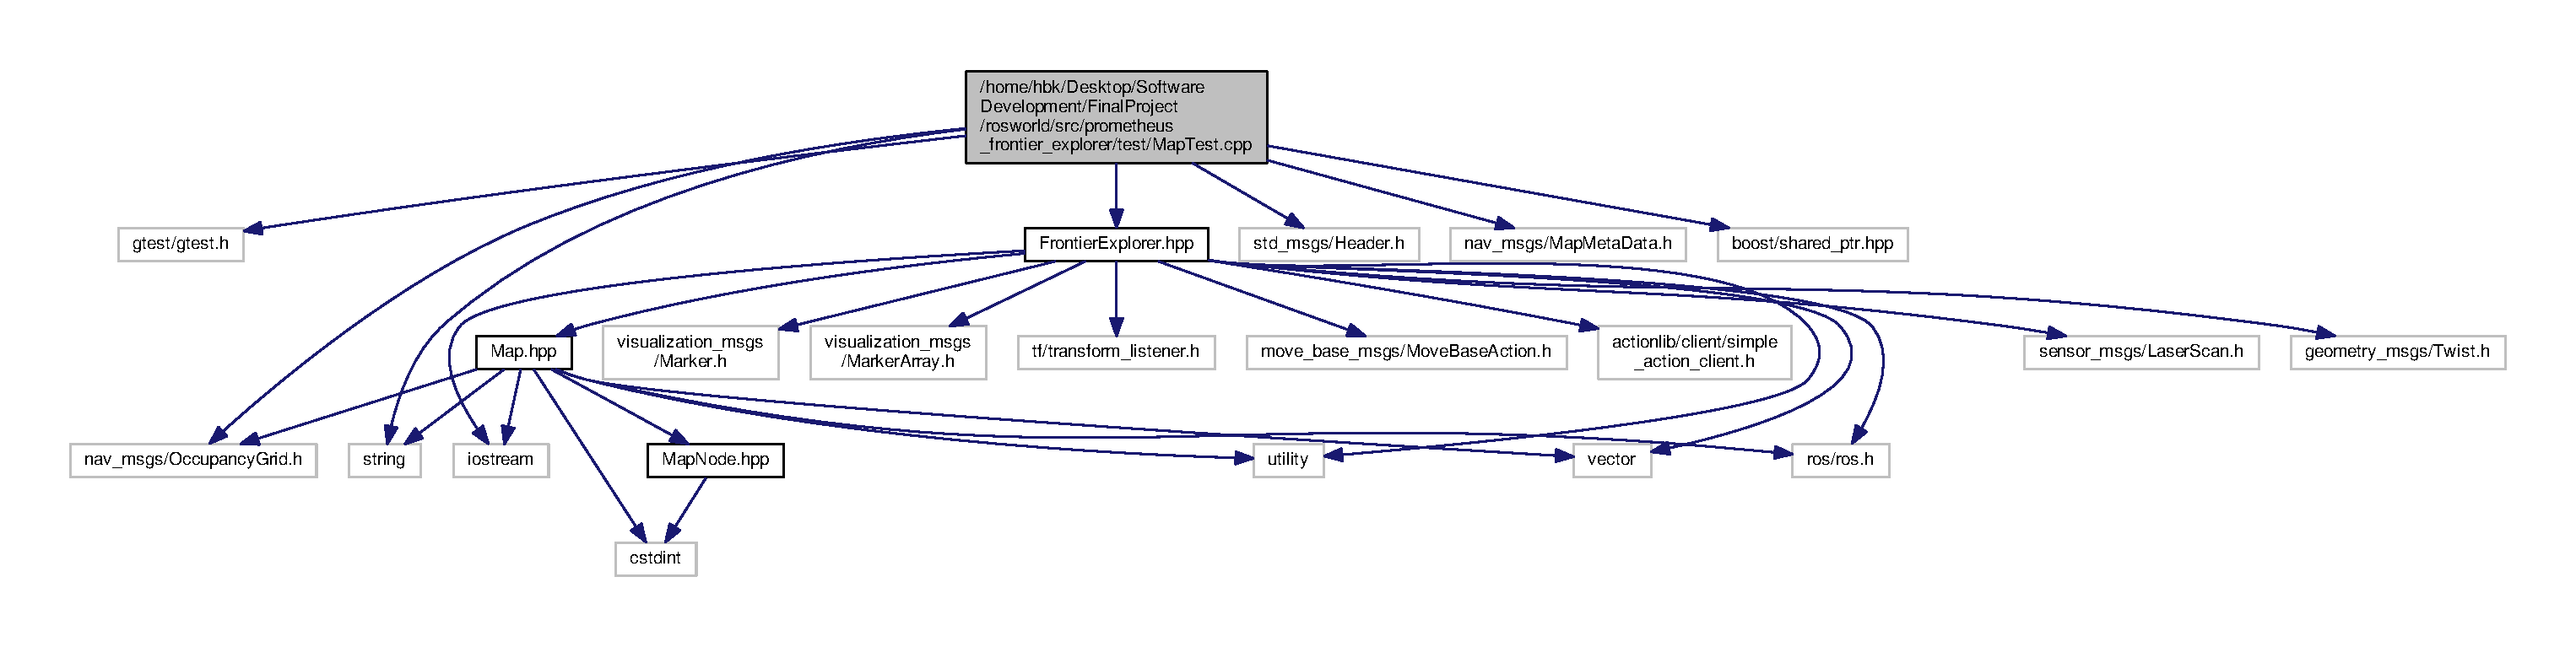
\includegraphics[width=350pt]{MapTest_8cpp__incl}
\end{center}
\end{figure}
\subsection*{Classes}
\begin{DoxyCompactItemize}
\item 
class \hyperlink{classMapTest}{Map\+Test}
\begin{DoxyCompactList}\small\item\em \hyperlink{classMapTest}{Map\+Test} Class. \end{DoxyCompactList}\end{DoxyCompactItemize}
\subsection*{Functions}
\begin{DoxyCompactItemize}
\item 
\hyperlink{MapTest_8cpp_a48516cf53985515c4dcd000280212d03}{T\+E\+S\+T\+\_\+F} (\hyperlink{classMapTest}{Map\+Test}, test\+Grid\+To\+Map)
\begin{DoxyCompactList}\small\item\em Test method to check callback and update map methods. \end{DoxyCompactList}\item 
\hyperlink{MapTest_8cpp_afde83efe218e988bfd62290baa2ecd87}{T\+E\+S\+T\+\_\+F} (\hyperlink{classMapTest}{Map\+Test}, test\+Get\+Frontiers)
\begin{DoxyCompactList}\small\item\em Test method to get frontiers from a dummy occupancy grid. \end{DoxyCompactList}\item 
\hyperlink{MapTest_8cpp_a82f1b521533be0ebfd5f64e1d72933e3}{T\+E\+S\+T\+\_\+F} (\hyperlink{classMapTest}{Map\+Test}, test\+Get\+Clusters)
\begin{DoxyCompactList}\small\item\em Test method to get clusters from a dummy occupancy grid. \end{DoxyCompactList}\item 
\hyperlink{MapTest_8cpp_a8127893a11d83ad34bc636f05218a1aa}{T\+E\+S\+T\+\_\+F} (\hyperlink{classMapTest}{Map\+Test}, test\+Get\+Cluster\+Centroids)
\begin{DoxyCompactList}\small\item\em Test method to get cluster centroids from a dummy grid. \end{DoxyCompactList}\item 
\hyperlink{MapTest_8cpp_a771e654137ec9f9e0cf480c3ae885c8e}{T\+E\+S\+T\+\_\+F} (\hyperlink{classMapTest}{Map\+Test}, test\+Set\+Map\+Set)
\begin{DoxyCompactList}\small\item\em Test set map flag method. \end{DoxyCompactList}\item 
\hyperlink{MapTest_8cpp_a5b0441d2f357d25be80ac599c7d0a045}{T\+E\+S\+T\+\_\+F} (\hyperlink{classMapTest}{Map\+Test}, test\+Set\+Map\+Height)
\begin{DoxyCompactList}\small\item\em Test set map height method. \end{DoxyCompactList}\item 
\hyperlink{MapTest_8cpp_a23fd04d04e553db3fc07550960aef979}{T\+E\+S\+T\+\_\+F} (\hyperlink{classMapTest}{Map\+Test}, test\+Set\+Map\+Width)
\begin{DoxyCompactList}\small\item\em Test set map width method. \end{DoxyCompactList}\item 
\hyperlink{MapTest_8cpp_a24e9ae1b1b2a4a6ea5e078631e3e0710}{T\+E\+S\+T\+\_\+F} (\hyperlink{classMapTest}{Map\+Test}, test\+Set\+Map\+Reso)
\begin{DoxyCompactList}\small\item\em Test set map resolution method. \end{DoxyCompactList}\item 
\hyperlink{MapTest_8cpp_afd738ab9a76fb25362fe5a408740b4b4}{T\+E\+S\+T\+\_\+F} (\hyperlink{classMapTest}{Map\+Test}, test\+Set\+Origin)
\begin{DoxyCompactList}\small\item\em Test set map origin method. \end{DoxyCompactList}\item 
\hyperlink{MapTest_8cpp_ab5f7d7d6e85445caf3e9d5e6fe6224dc}{T\+E\+S\+T\+\_\+F} (\hyperlink{classMapTest}{Map\+Test}, test\+Get\+Map\+Set)
\begin{DoxyCompactList}\small\item\em Test get map flag method. \end{DoxyCompactList}\item 
\hyperlink{MapTest_8cpp_a1cdee4ee5f9229d6779b70bc4c483207}{T\+E\+S\+T\+\_\+F} (\hyperlink{classMapTest}{Map\+Test}, test\+Get\+Map\+Height)
\begin{DoxyCompactList}\small\item\em Test get map height method. \end{DoxyCompactList}\item 
\hyperlink{MapTest_8cpp_a336ba319cdc8be4892ec713a70866db2}{T\+E\+S\+T\+\_\+F} (\hyperlink{classMapTest}{Map\+Test}, test\+Get\+Map\+Width)
\begin{DoxyCompactList}\small\item\em Test get map width method. \end{DoxyCompactList}\item 
\hyperlink{MapTest_8cpp_a62be965611c07d197bf712b43312b0ba}{T\+E\+S\+T\+\_\+F} (\hyperlink{classMapTest}{Map\+Test}, test\+Get\+Map\+Reso)
\begin{DoxyCompactList}\small\item\em Test get map resolution method. \end{DoxyCompactList}\item 
\hyperlink{MapTest_8cpp_ac4a90c6c66f3fc25fdcca6ccf15c8a94}{T\+E\+S\+T\+\_\+F} (\hyperlink{classMapTest}{Map\+Test}, test\+Get\+Origin)
\begin{DoxyCompactList}\small\item\em Test get map origin method. \end{DoxyCompactList}\end{DoxyCompactItemize}


\subsection{Detailed Description}
Test for \hyperlink{classMap}{Map} class file. 

\begin{DoxyAuthor}{Author}
Harsh Kakashaniya and Rohitkrishna Nambiar 
\end{DoxyAuthor}
\begin{DoxyDate}{Date}
12/04/2018 
\end{DoxyDate}
\begin{DoxyVersion}{Version}
1.\+0 
\end{DoxyVersion}
\begin{DoxyCopyright}{Copyright}
B\+SD 3-\/\+Clause
\end{DoxyCopyright}
\hypertarget{MapTest_8cpp_DESCRIPTION}{}\subsection{D\+E\+S\+C\+R\+I\+P\+T\+I\+ON}\label{MapTest_8cpp_DESCRIPTION}
Test implementation for \hyperlink{classMap}{Map} class 

\subsection{Function Documentation}
\index{Map\+Test.\+cpp@{Map\+Test.\+cpp}!T\+E\+S\+T\+\_\+F@{T\+E\+S\+T\+\_\+F}}
\index{T\+E\+S\+T\+\_\+F@{T\+E\+S\+T\+\_\+F}!Map\+Test.\+cpp@{Map\+Test.\+cpp}}
\subsubsection[{\texorpdfstring{T\+E\+S\+T\+\_\+\+F(\+Map\+Test, test\+Grid\+To\+Map)}{TEST_F(MapTest, testGridToMap)}}]{\setlength{\rightskip}{0pt plus 5cm}T\+E\+S\+T\+\_\+F (
\begin{DoxyParamCaption}
\item[{{\bf Map\+Test}}]{, }
\item[{test\+Grid\+To\+Map}]{}
\end{DoxyParamCaption}
)}\hypertarget{MapTest_8cpp_a48516cf53985515c4dcd000280212d03}{}\label{MapTest_8cpp_a48516cf53985515c4dcd000280212d03}


Test method to check callback and update map methods. 


\begin{DoxyParams}{Parameters}
{\em none} & \\
\hline
\end{DoxyParams}
\begin{DoxyReturn}{Returns}
none 
\end{DoxyReturn}
\index{Map\+Test.\+cpp@{Map\+Test.\+cpp}!T\+E\+S\+T\+\_\+F@{T\+E\+S\+T\+\_\+F}}
\index{T\+E\+S\+T\+\_\+F@{T\+E\+S\+T\+\_\+F}!Map\+Test.\+cpp@{Map\+Test.\+cpp}}
\subsubsection[{\texorpdfstring{T\+E\+S\+T\+\_\+\+F(\+Map\+Test, test\+Get\+Frontiers)}{TEST_F(MapTest, testGetFrontiers)}}]{\setlength{\rightskip}{0pt plus 5cm}T\+E\+S\+T\+\_\+F (
\begin{DoxyParamCaption}
\item[{{\bf Map\+Test}}]{, }
\item[{test\+Get\+Frontiers}]{}
\end{DoxyParamCaption}
)}\hypertarget{MapTest_8cpp_afde83efe218e988bfd62290baa2ecd87}{}\label{MapTest_8cpp_afde83efe218e988bfd62290baa2ecd87}


Test method to get frontiers from a dummy occupancy grid. 


\begin{DoxyParams}{Parameters}
{\em none} & \\
\hline
\end{DoxyParams}
\begin{DoxyReturn}{Returns}
none 
\end{DoxyReturn}
\index{Map\+Test.\+cpp@{Map\+Test.\+cpp}!T\+E\+S\+T\+\_\+F@{T\+E\+S\+T\+\_\+F}}
\index{T\+E\+S\+T\+\_\+F@{T\+E\+S\+T\+\_\+F}!Map\+Test.\+cpp@{Map\+Test.\+cpp}}
\subsubsection[{\texorpdfstring{T\+E\+S\+T\+\_\+\+F(\+Map\+Test, test\+Get\+Clusters)}{TEST_F(MapTest, testGetClusters)}}]{\setlength{\rightskip}{0pt plus 5cm}T\+E\+S\+T\+\_\+F (
\begin{DoxyParamCaption}
\item[{{\bf Map\+Test}}]{, }
\item[{test\+Get\+Clusters}]{}
\end{DoxyParamCaption}
)}\hypertarget{MapTest_8cpp_a82f1b521533be0ebfd5f64e1d72933e3}{}\label{MapTest_8cpp_a82f1b521533be0ebfd5f64e1d72933e3}


Test method to get clusters from a dummy occupancy grid. 


\begin{DoxyParams}{Parameters}
{\em none} & \\
\hline
\end{DoxyParams}
\begin{DoxyReturn}{Returns}
none 
\end{DoxyReturn}
\index{Map\+Test.\+cpp@{Map\+Test.\+cpp}!T\+E\+S\+T\+\_\+F@{T\+E\+S\+T\+\_\+F}}
\index{T\+E\+S\+T\+\_\+F@{T\+E\+S\+T\+\_\+F}!Map\+Test.\+cpp@{Map\+Test.\+cpp}}
\subsubsection[{\texorpdfstring{T\+E\+S\+T\+\_\+\+F(\+Map\+Test, test\+Get\+Cluster\+Centroids)}{TEST_F(MapTest, testGetClusterCentroids)}}]{\setlength{\rightskip}{0pt plus 5cm}T\+E\+S\+T\+\_\+F (
\begin{DoxyParamCaption}
\item[{{\bf Map\+Test}}]{, }
\item[{test\+Get\+Cluster\+Centroids}]{}
\end{DoxyParamCaption}
)}\hypertarget{MapTest_8cpp_a8127893a11d83ad34bc636f05218a1aa}{}\label{MapTest_8cpp_a8127893a11d83ad34bc636f05218a1aa}


Test method to get cluster centroids from a dummy grid. 


\begin{DoxyParams}{Parameters}
{\em none} & \\
\hline
\end{DoxyParams}
\begin{DoxyReturn}{Returns}
none 
\end{DoxyReturn}
\index{Map\+Test.\+cpp@{Map\+Test.\+cpp}!T\+E\+S\+T\+\_\+F@{T\+E\+S\+T\+\_\+F}}
\index{T\+E\+S\+T\+\_\+F@{T\+E\+S\+T\+\_\+F}!Map\+Test.\+cpp@{Map\+Test.\+cpp}}
\subsubsection[{\texorpdfstring{T\+E\+S\+T\+\_\+\+F(\+Map\+Test, test\+Set\+Map\+Set)}{TEST_F(MapTest, testSetMapSet)}}]{\setlength{\rightskip}{0pt plus 5cm}T\+E\+S\+T\+\_\+F (
\begin{DoxyParamCaption}
\item[{{\bf Map\+Test}}]{, }
\item[{test\+Set\+Map\+Set}]{}
\end{DoxyParamCaption}
)}\hypertarget{MapTest_8cpp_a771e654137ec9f9e0cf480c3ae885c8e}{}\label{MapTest_8cpp_a771e654137ec9f9e0cf480c3ae885c8e}


Test set map flag method. 


\begin{DoxyParams}{Parameters}
{\em none} & \\
\hline
\end{DoxyParams}
\begin{DoxyReturn}{Returns}
none 
\end{DoxyReturn}
\index{Map\+Test.\+cpp@{Map\+Test.\+cpp}!T\+E\+S\+T\+\_\+F@{T\+E\+S\+T\+\_\+F}}
\index{T\+E\+S\+T\+\_\+F@{T\+E\+S\+T\+\_\+F}!Map\+Test.\+cpp@{Map\+Test.\+cpp}}
\subsubsection[{\texorpdfstring{T\+E\+S\+T\+\_\+\+F(\+Map\+Test, test\+Set\+Map\+Height)}{TEST_F(MapTest, testSetMapHeight)}}]{\setlength{\rightskip}{0pt plus 5cm}T\+E\+S\+T\+\_\+F (
\begin{DoxyParamCaption}
\item[{{\bf Map\+Test}}]{, }
\item[{test\+Set\+Map\+Height}]{}
\end{DoxyParamCaption}
)}\hypertarget{MapTest_8cpp_a5b0441d2f357d25be80ac599c7d0a045}{}\label{MapTest_8cpp_a5b0441d2f357d25be80ac599c7d0a045}


Test set map height method. 


\begin{DoxyParams}{Parameters}
{\em none} & \\
\hline
\end{DoxyParams}
\begin{DoxyReturn}{Returns}
none 
\end{DoxyReturn}
\index{Map\+Test.\+cpp@{Map\+Test.\+cpp}!T\+E\+S\+T\+\_\+F@{T\+E\+S\+T\+\_\+F}}
\index{T\+E\+S\+T\+\_\+F@{T\+E\+S\+T\+\_\+F}!Map\+Test.\+cpp@{Map\+Test.\+cpp}}
\subsubsection[{\texorpdfstring{T\+E\+S\+T\+\_\+\+F(\+Map\+Test, test\+Set\+Map\+Width)}{TEST_F(MapTest, testSetMapWidth)}}]{\setlength{\rightskip}{0pt plus 5cm}T\+E\+S\+T\+\_\+F (
\begin{DoxyParamCaption}
\item[{{\bf Map\+Test}}]{, }
\item[{test\+Set\+Map\+Width}]{}
\end{DoxyParamCaption}
)}\hypertarget{MapTest_8cpp_a23fd04d04e553db3fc07550960aef979}{}\label{MapTest_8cpp_a23fd04d04e553db3fc07550960aef979}


Test set map width method. 


\begin{DoxyParams}{Parameters}
{\em none} & \\
\hline
\end{DoxyParams}
\begin{DoxyReturn}{Returns}
none 
\end{DoxyReturn}
\index{Map\+Test.\+cpp@{Map\+Test.\+cpp}!T\+E\+S\+T\+\_\+F@{T\+E\+S\+T\+\_\+F}}
\index{T\+E\+S\+T\+\_\+F@{T\+E\+S\+T\+\_\+F}!Map\+Test.\+cpp@{Map\+Test.\+cpp}}
\subsubsection[{\texorpdfstring{T\+E\+S\+T\+\_\+\+F(\+Map\+Test, test\+Set\+Map\+Reso)}{TEST_F(MapTest, testSetMapReso)}}]{\setlength{\rightskip}{0pt plus 5cm}T\+E\+S\+T\+\_\+F (
\begin{DoxyParamCaption}
\item[{{\bf Map\+Test}}]{, }
\item[{test\+Set\+Map\+Reso}]{}
\end{DoxyParamCaption}
)}\hypertarget{MapTest_8cpp_a24e9ae1b1b2a4a6ea5e078631e3e0710}{}\label{MapTest_8cpp_a24e9ae1b1b2a4a6ea5e078631e3e0710}


Test set map resolution method. 


\begin{DoxyParams}{Parameters}
{\em none} & \\
\hline
\end{DoxyParams}
\begin{DoxyReturn}{Returns}
none 
\end{DoxyReturn}
\index{Map\+Test.\+cpp@{Map\+Test.\+cpp}!T\+E\+S\+T\+\_\+F@{T\+E\+S\+T\+\_\+F}}
\index{T\+E\+S\+T\+\_\+F@{T\+E\+S\+T\+\_\+F}!Map\+Test.\+cpp@{Map\+Test.\+cpp}}
\subsubsection[{\texorpdfstring{T\+E\+S\+T\+\_\+\+F(\+Map\+Test, test\+Set\+Origin)}{TEST_F(MapTest, testSetOrigin)}}]{\setlength{\rightskip}{0pt plus 5cm}T\+E\+S\+T\+\_\+F (
\begin{DoxyParamCaption}
\item[{{\bf Map\+Test}}]{, }
\item[{test\+Set\+Origin}]{}
\end{DoxyParamCaption}
)}\hypertarget{MapTest_8cpp_afd738ab9a76fb25362fe5a408740b4b4}{}\label{MapTest_8cpp_afd738ab9a76fb25362fe5a408740b4b4}


Test set map origin method. 


\begin{DoxyParams}{Parameters}
{\em none} & \\
\hline
\end{DoxyParams}
\begin{DoxyReturn}{Returns}
none 
\end{DoxyReturn}
\index{Map\+Test.\+cpp@{Map\+Test.\+cpp}!T\+E\+S\+T\+\_\+F@{T\+E\+S\+T\+\_\+F}}
\index{T\+E\+S\+T\+\_\+F@{T\+E\+S\+T\+\_\+F}!Map\+Test.\+cpp@{Map\+Test.\+cpp}}
\subsubsection[{\texorpdfstring{T\+E\+S\+T\+\_\+\+F(\+Map\+Test, test\+Get\+Map\+Set)}{TEST_F(MapTest, testGetMapSet)}}]{\setlength{\rightskip}{0pt plus 5cm}T\+E\+S\+T\+\_\+F (
\begin{DoxyParamCaption}
\item[{{\bf Map\+Test}}]{, }
\item[{test\+Get\+Map\+Set}]{}
\end{DoxyParamCaption}
)}\hypertarget{MapTest_8cpp_ab5f7d7d6e85445caf3e9d5e6fe6224dc}{}\label{MapTest_8cpp_ab5f7d7d6e85445caf3e9d5e6fe6224dc}


Test get map flag method. 


\begin{DoxyParams}{Parameters}
{\em none} & \\
\hline
\end{DoxyParams}
\begin{DoxyReturn}{Returns}
none 
\end{DoxyReturn}
\index{Map\+Test.\+cpp@{Map\+Test.\+cpp}!T\+E\+S\+T\+\_\+F@{T\+E\+S\+T\+\_\+F}}
\index{T\+E\+S\+T\+\_\+F@{T\+E\+S\+T\+\_\+F}!Map\+Test.\+cpp@{Map\+Test.\+cpp}}
\subsubsection[{\texorpdfstring{T\+E\+S\+T\+\_\+\+F(\+Map\+Test, test\+Get\+Map\+Height)}{TEST_F(MapTest, testGetMapHeight)}}]{\setlength{\rightskip}{0pt plus 5cm}T\+E\+S\+T\+\_\+F (
\begin{DoxyParamCaption}
\item[{{\bf Map\+Test}}]{, }
\item[{test\+Get\+Map\+Height}]{}
\end{DoxyParamCaption}
)}\hypertarget{MapTest_8cpp_a1cdee4ee5f9229d6779b70bc4c483207}{}\label{MapTest_8cpp_a1cdee4ee5f9229d6779b70bc4c483207}


Test get map height method. 


\begin{DoxyParams}{Parameters}
{\em none} & \\
\hline
\end{DoxyParams}
\begin{DoxyReturn}{Returns}
none 
\end{DoxyReturn}
\index{Map\+Test.\+cpp@{Map\+Test.\+cpp}!T\+E\+S\+T\+\_\+F@{T\+E\+S\+T\+\_\+F}}
\index{T\+E\+S\+T\+\_\+F@{T\+E\+S\+T\+\_\+F}!Map\+Test.\+cpp@{Map\+Test.\+cpp}}
\subsubsection[{\texorpdfstring{T\+E\+S\+T\+\_\+\+F(\+Map\+Test, test\+Get\+Map\+Width)}{TEST_F(MapTest, testGetMapWidth)}}]{\setlength{\rightskip}{0pt plus 5cm}T\+E\+S\+T\+\_\+F (
\begin{DoxyParamCaption}
\item[{{\bf Map\+Test}}]{, }
\item[{test\+Get\+Map\+Width}]{}
\end{DoxyParamCaption}
)}\hypertarget{MapTest_8cpp_a336ba319cdc8be4892ec713a70866db2}{}\label{MapTest_8cpp_a336ba319cdc8be4892ec713a70866db2}


Test get map width method. 


\begin{DoxyParams}{Parameters}
{\em none} & \\
\hline
\end{DoxyParams}
\begin{DoxyReturn}{Returns}
none 
\end{DoxyReturn}
\index{Map\+Test.\+cpp@{Map\+Test.\+cpp}!T\+E\+S\+T\+\_\+F@{T\+E\+S\+T\+\_\+F}}
\index{T\+E\+S\+T\+\_\+F@{T\+E\+S\+T\+\_\+F}!Map\+Test.\+cpp@{Map\+Test.\+cpp}}
\subsubsection[{\texorpdfstring{T\+E\+S\+T\+\_\+\+F(\+Map\+Test, test\+Get\+Map\+Reso)}{TEST_F(MapTest, testGetMapReso)}}]{\setlength{\rightskip}{0pt plus 5cm}T\+E\+S\+T\+\_\+F (
\begin{DoxyParamCaption}
\item[{{\bf Map\+Test}}]{, }
\item[{test\+Get\+Map\+Reso}]{}
\end{DoxyParamCaption}
)}\hypertarget{MapTest_8cpp_a62be965611c07d197bf712b43312b0ba}{}\label{MapTest_8cpp_a62be965611c07d197bf712b43312b0ba}


Test get map resolution method. 


\begin{DoxyParams}{Parameters}
{\em none} & \\
\hline
\end{DoxyParams}
\begin{DoxyReturn}{Returns}
none 
\end{DoxyReturn}
\index{Map\+Test.\+cpp@{Map\+Test.\+cpp}!T\+E\+S\+T\+\_\+F@{T\+E\+S\+T\+\_\+F}}
\index{T\+E\+S\+T\+\_\+F@{T\+E\+S\+T\+\_\+F}!Map\+Test.\+cpp@{Map\+Test.\+cpp}}
\subsubsection[{\texorpdfstring{T\+E\+S\+T\+\_\+\+F(\+Map\+Test, test\+Get\+Origin)}{TEST_F(MapTest, testGetOrigin)}}]{\setlength{\rightskip}{0pt plus 5cm}T\+E\+S\+T\+\_\+F (
\begin{DoxyParamCaption}
\item[{{\bf Map\+Test}}]{, }
\item[{test\+Get\+Origin}]{}
\end{DoxyParamCaption}
)}\hypertarget{MapTest_8cpp_ac4a90c6c66f3fc25fdcca6ccf15c8a94}{}\label{MapTest_8cpp_ac4a90c6c66f3fc25fdcca6ccf15c8a94}


Test get map origin method. 


\begin{DoxyParams}{Parameters}
{\em none} & \\
\hline
\end{DoxyParams}
\begin{DoxyReturn}{Returns}
none 
\end{DoxyReturn}

%--- End generated contents ---

% Index
\backmatter
\newpage
\phantomsection
\clearemptydoublepage
\addcontentsline{toc}{chapter}{Index}
\printindex

\end{document}
